\documentclass[12pt]{report}
\usepackage{graphicx}
\usepackage{amsmath}
\usepackage{float}
\usepackage{titlesec}
\usepackage{subcaption}
\usepackage{caption}
\usepackage[a4paper, left=2.5cm, right=2.5cm, top=2.5cm, bottom=2.5cm]{geometry}
\usepackage{fancyvrb}
\usepackage[utf8]{inputenc}
\usepackage{geometry}
\usepackage{setspace}
\usepackage{titling}
\usepackage{lmodern}
\usepackage{ragged2e}
\usepackage{array}
\usepackage{tocloft}
\setlength{\cftfignumwidth}{3.5em}
\geometry{
 a4paper,
 total={160mm,247mm},
 left=25mm,
 top=25mm,
}

\pagenumbering{gobble}
\setstretch{1.15} % Slightly reduced

\DefineVerbatimEnvironment{boxedverbatim}{Verbatim}{%
    frame=single,
    framesep=2mm,
    fontsize=\small,
    commandchars=\\\{\}
}

% Number figures as <chapter>.<section>.<figure>
\renewcommand\thefigure{\thechapter.\thesection.\arabic{figure}}
\counterwithin{figure}{section}

\titlelabel{\thetitle.\quad}

\setlength{\parskip}{1em}
\setlength{\parindent}{0pt}


\begin{document}
% Logos and header
\vspace*{-1.5cm} % Adjust this to move content up if needed
\begin{minipage}{0.25\textwidth}
  
\includegraphics[width=2.8cm]{insat_logo.png}
\end{minipage}%
\begin{minipage}{0.5\textwidth}
  \centering
  \small\textbf{TUNISIAN REPUBLIC} \\
  \footnotesize Ministry of Higher Education and Scientific Research \\
  \footnotesize University of Carthage \\
  \small\textbf{National Institute of Applied Sciences and Technology}
\end{minipage}%
\begin{minipage}{0.25\textwidth}
  \raggedleft
  
\includegraphics[width=2.8cm]{ucar_logo.png}
\end{minipage}

\vspace{0.4cm}

% Title
\begin{center}
  \large\textbf{End of Year Project} \\[0.2cm]
  \small submitted as part of the \\
  \textbf{End of Year Project Report} \\
  \small Specialty: \textbf{Software Engineering}
\end{center}

\vspace{0.4cm}

% Project Title + App Logo
\begin{center}
  \textbf{\large AI-powered Mobile Application for\\ Breathing Sound Analysis and Disease Detection}
  
  \vspace{0.3cm}
  
\includegraphics[width=2.5cm]{images/UI_Screenshots/logo_filled.png}
\end{center}

\vspace{0.5cm}

% Authors
\begin{center}
  \small Prepared by \\[0.1cm]
  \normalsize\textbf{Ahmed SILINI} \\
  \normalsize\textbf{Ghassen CHERIF} \\
  \normalsize\textbf{Mohamed Aziz BALTI}
\end{center}

\vspace{0.5cm}

% Defense info
\begin{center}
  \small Defended on the \textbf{4th of May 2025} \\
  \small in front of a jury composed of:
\end{center}

\vspace{0.3cm}

\begin{center}
\begin{tabular}{m{5.5cm} m{5.5cm}}
\centering\arraybackslash \small\textbf{Dr. Sana HAMDI} & \centering\arraybackslash \small\textbf{Dr. Wided MILED} \\
\centering\arraybackslash \footnotesize Supervisor & \centering\arraybackslash \footnotesize Examiner \\
\end{tabular}
\end{center}

\vspace{0.4cm}

% Academic year
\begin{center}
  \small Academic year: \textbf{2024 / 2025}
\end{center}

\vspace*{\fill} % Fills remaining space to push content to top
\chapter*{Dedication}

\begin{center}
\begin{minipage}{0.9\textwidth}
\itshape
This project is dedicated with deep gratitude and respect to those who have stood beside us throughout this journey.

\vspace{0.4cm}

To our families — your unwavering love, support, and encouragement have been the pillars upon which we’ve built not only this work, but our growth and perseverance. Your sacrifices, patience, and belief in our potential gave us strength when we needed it most.

\vspace{0.4cm}

To our supervisor, \textbf{Dr. Sana HAMDI} — thank you for your insightful guidance, constructive feedback, and constant encouragement. Your trust in our abilities pushed us to do better and take ownership of our work. We are truly grateful for your mentorship and your commitment to helping us succeed.

\vspace{0.4cm}

To our professors and the faculty at \textbf{INSAT}, thank you for shaping our knowledge, skills, and mindset over the past years. Your dedication to education and innovation has inspired us to pursue excellence in everything we do.

\vspace{0.4cm}

Finally, to each other — for the collaboration, resilience, and shared passion that carried this project forward. This work is a testament to teamwork and shared vision.

\vspace{0.4cm}

With heartfelt appreciation, \\
Ahmed SILINI \\
Ghassen CHERIF \\
Mohamed Aziz BALTI
\end{minipage}
\end{center}

\newpage
\tableofcontents
\thispagestyle{empty}
\newpage



\chapter*{List of Acronyms}
\addcontentsline{toc}{chapter}{List of Acronyms}
\addcontentsline{toc}{chapter}{List of Acronyms}

\begin{tabbing}

\hspace{2cm} \= \kill
AI \> Artificial Intelligence \\
COPD \> Chronic Obstructive Pulmonary Disease \\
COVID-19 \> Coronavirus Disease 2019 \\
CLAP \> Contrastive Learning Audio Processing \\
RAG \> Retrieval-Augmented Generation \\
LLM \> Large Language Model \\
CRISP-DM \> Cross-Industry Standard Process for Data Mining \\
RNN \> Recurrent Neural Network \\
CNN \> Convolutional Neural Network \\
DL \> Deep Learning \\
LlaMa \> Large Language Model Meta AI \\
BERT \> Bidirectional Encoder Representations from Transformers \\
BGE \> BERT Generated Embeddings \\
MRR \> Mean Reciprocal Rank \\
MAP \> Mean Average Precision \\
UCD \> User-Centered Design \\
BaaS \> Backend-as-a-Service \\
WHO \> World Health Organization \\
CDC \> Centers for Disease Control and Prevention \\
API \> Application Programming Interface \\
REST \> Representational State Transfer \\
UI \> User Interface \\
HTTPS \> Hypertext Transfer Protocol Secure \\
JSON \> JavaScript Object Notation \\
iOS \> iPhone Operating System \\
VS Code \> Visual Studio Code \\

\end{tabbing}


\addcontentsline{toc}{section}{List of Figures}
\listoffigures


\newpage


\chapter*{General Introduction}
\addcontentsline{toc}{section}{General Introduction}

The rapid evolution of artificial intelligence (AI) and mobile technologies has brought transformative changes across multiple domains, including healthcare. These advancements are now enabling the design of intelligent systems that support early disease detection, remote monitoring, and accessible diagnostics. One area of growing relevance is respiratory health, particularly in light of the increased attention to respiratory diseases following the COVID-19 pandemic and the continued burden of chronic conditions such as asthma, chronic obstructive pulmonary disease (COPD), and sleep apnea.

Despite the prevalence of such conditions, access to timely and affordable respiratory screening remains limited in many parts of the world. Specialized medical equipment and trained professionals are often required to conduct auscultation and interpret respiratory anomalies. This reality poses a significant barrier to early detection and long-term monitoring—two factors that are critical to improving patient outcomes. The proliferation of smartphones, however, opens new opportunities for building accessible, AI-powered health tools that can reach broader populations.

This end-of-year project seeks to address this challenge by designing and implementing a mobile application capable of analyzing breathing sounds and providing AI-assisted respiratory diagnostics. The system enables users to record audio samples using a smartphone microphone, which are then processed using machine learning models trained to classify respiratory anomalies such as wheezing, crackles, and rhonchi. Based on the classification results, the system offers a preliminary diagnostic suggestion. To enhance usability and trust, a conversational AI assistant is also integrated—allowing users to ask questions, receive explanations, and obtain medically grounded feedback.

The core objective of the project is to provide a portable and intelligent solution for respiratory disease detection, one that combines ease of use, technical robustness, and medical relevance. Achieving this goal involves contributions across multiple areas of computer science, including mobile development, signal processing, deep learning, backend architecture, and natural language processing.

The mobile application is built using a cross-platform framework, ensuring compatibility with both Android and iOS devices. It includes modules for secure user authentication, audio recording, and diagnosis history tracking. The backend infrastructure, powered by a backend-as-a-service platform, supports encrypted data storage, API integration, and serverless functions for model inference. On the AI side, two main components are developed: (1) a contrastive learning model (CLAP) for respiratory sound classification, and (2) a lightweight retrieval-augmented generation (RAG) chatbot based on a quantized language model. These components are trained on publicly available datasets and fine-tuned to deliver fast, accurate, and explainable results to end users.

Beyond implementation, this report provides a structured exploration of the project lifecycle, from the initial definition of objectives to system evaluation. Chapter 1 introduces the general context, the underlying problem, and the proposed solution. Chapter 2 outlines the foundational concepts that support the system, including respiratory anomalies, deep learning principles, and mobile development strategies. Chapter 3 presents a review of related work in respiratory diagnostics and medical chatbots. Chapters 4 and 5 detail the application of the CRISP-DM methodology to both the classification model and the AI assistant. Chapter 6 focuses on implementation, highlighting system architecture, mobile development, backend integration, and the tools used.

Through this interdisciplinary work, we aim not only to demonstrate the feasibility of smartphone-based respiratory diagnostics, but also to contribute to the broader field of AI for public health. By combining modern machine learning techniques with accessible mobile interfaces, the project aspires to bring preliminary respiratory screening closer to users—anytime, anywhere.


\chapter{1. General Context}
\section*{1. General Context}

Respiratory diseases, such as asthma, chronic obstructive pulmonary disease (COPD), and bronchitis, remain among the most common and impactful health challenges globally. Early detection and effective diagnosis are essential for reducing complications and improving patient outcomes. Traditionally, respiratory assessment relies heavily on auscultation—the process of listening to lung sounds through a stethoscope. While widely practiced, this technique depends greatly on clinical expertise and is inherently subjective.

As digital health tools become more accessible, especially through smartphones, there is growing potential to transform the way respiratory conditions are detected and monitored. In particular, the use of Artificial Intelligence (AI) enables automated analysis of lung sounds and medical data, providing faster and potentially more accurate support for both patients and clinicians.

This project introduces a mobile application that empowers users to monitor their respiratory health at home. The app allows users to record breathing sounds using their phone’s microphone and upload personal medical documents (e.g., prescriptions, symptom reports, or discharge summaries). Through secure and privacy-preserving AI techniques, these inputs are analyzed to detect respiratory anomalies and provide informed assistance.

\subsection*{1.1 Project Background and Objectives}

\subsubsection*{1.1.1 Project Context}

The idea for this system is rooted in the limitations of traditional diagnostic tools and the underutilization of available clinical information. Public datasets, such as the ICBHI 2017 Respiratory Sound Database, have demonstrated the feasibility of using machine learning for automated respiratory sound classification. However, most existing approaches focus solely on audio data, ignoring valuable contextual clues that could be derived from a patient's medical history or symptoms.

This project builds upon these foundations by embracing a multimodal approach. It combines the power of deep audio models with textual understanding to interpret both lung sounds and patient-specific metadata. The mobile app becomes a bridge between clinical-grade respiratory screening and user-friendly, accessible diagnostics.

\subsubsection*{1.1.2 Problem Statement}

Current solutions for respiratory anomaly detection face several limitations:
\begin{itemize}
    \item \textbf{Single Modality Focus:} Many existing tools rely exclusively on sound data, overlooking important contextual information.
    \item \textbf{Subjectivity in Diagnosis:} Manual auscultation is prone to human error and variability between clinicians.
    \item \textbf{Lack of Interpretability:} Users often receive a diagnosis or prediction without any explanation or follow-up guidance.
    \item \textbf{Limited Accessibility:} Clinical tools are often not available outside hospitals or specialized environments.
\end{itemize}

This project addresses the following key question:

\textit{“How can we build an AI-powered mobile application that combines user-recorded lung sounds with clinical records to detect respiratory anomalies and provide intelligent, interactive feedback?”}

\subsubsection*{1.1.3 Proposed Solution}

We propose an integrated, user-friendly mobile application that performs end-to-end respiratory analysis using multimodal AI. The system operates as follows:

\begin{itemize}
    \item \textbf{User Interaction:} The user records their breathing sounds through the app and optionally uploads medical documentation in PDF format.
    \item \textbf{Multimodal Embedding:} A pretrained CLAP (Contrastive Language-Audio Pretraining) model is used to embed both the audio signal and extracted text from the medical documents into a shared latent space, capturing a holistic representation of the patient's condition.
    \item \textbf{Respiratory Anomaly Detection:} Using these embeddings, the model classifies the type of lung sound (e.g., \textit{normal}, \textit{wheeze}, \textit{crackle}, or \textit{both}).
    \item \textbf{Clinical Reasoning:} The app then sends the output to a Large Language Model (LLM), which, supported by a Retrieval-Augmented Generation (RAG) system, infers possible underlying conditions and provides medically-informed responses.
    \item \textbf{Conversational Assistant:} The LLM acts as a virtual assistant that explains results, suggests next steps, and answers follow-up questions, helping users make sense of their health status.
    \item \textbf{Privacy and Security:} All user data is handled with strong encryption and processed locally or on secure servers in compliance with healthcare data regulations.
\end{itemize}

By combining sound interpretation, contextual analysis, and conversational intelligence in a single mobile interface, this solution aims to democratize respiratory diagnostics. It supports users with accessible insights while maintaining clinical relevance, and ultimately enhances both early detection and user understanding in a safe, secure manner.

\section{Project Methodology}
\subsection{Methodology: CRISP-DM Methodology}

During our project, we chose to adopt the \textit{Cross-Industry Standard Process for Data Mining (CRISP-DM)} methodology. CRISP-DM is a well-known framework for data mining and ML projects. It offers detailed steps that cover the entirety of the project flow, from its business understanding to its deployment. The key steps defined by this framework that we went by are illustrated in Figure~\ref{fig:crisp-dm} and are as follows:

\begin{itemize}
    \item \textbf{Business Understanding:} This includes defining the business needs and understanding the issues we are addressing with our project. This is also where we define our business goals and requirements.

    \item \textbf{Data Understanding:} This step includes the exploration and analysis of our available data, highlighting its different characteristics, identifying any potential biases it may have, and understanding our acquired data and the preprocessing steps we need to get it.

    \item \textbf{Data Preparation:} This is the step where we apply different preprocessing techniques to our acquired data. This might include preparing the data for modeling, ensuring it has suitable formats, etc.

    \item \textbf{Modeling:} This consists of selecting appropriate models for our task, training and fine-tuning them using the prepared data, and experimenting with different architectures, hyperparameters, and optimization techniques to enhance model performance.

    \item \textbf{Evaluation:} In this step, we evaluate the performance of the models using appropriate metrics for the specific tasks, and we assess their effectiveness in those tasks.

    \item \textbf{Deployment:} This step is dedicated to studying real-life scenarios where our chosen model might be needed, potentially leading to its deployment to make it available to users.
\end{itemize}

\begin{figure}[htbp]
    \centering
    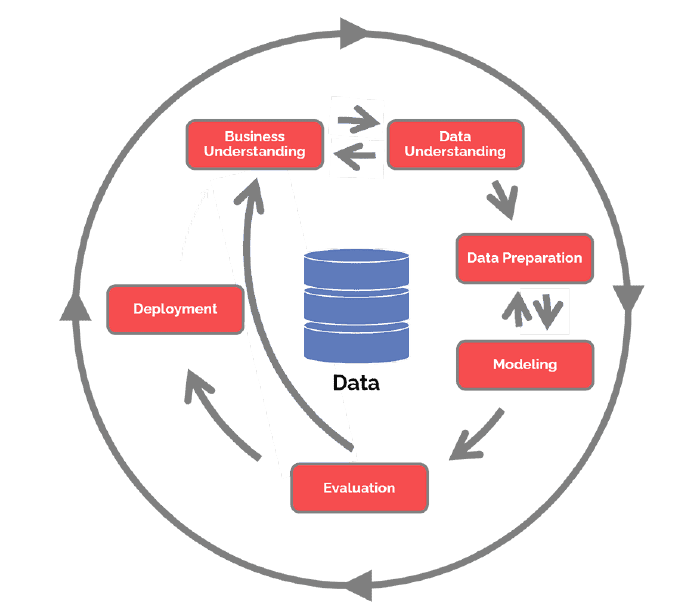
\includegraphics[width=0.5\textwidth]{images/crisp-dm-diagram.png}
    \caption{The different steps of the CRISP-DM methodology.}
    \label{fig:crisp-dm}
\end{figure}

\subsection{Project Planning (Gantt Chart)}
Figure~\ref{fig:gantt-chart} illustrates the Gantt diagram detailing our project timeline from April 24th, to Mai, 18th.

\begin{figure}[htbp]
    \centering
    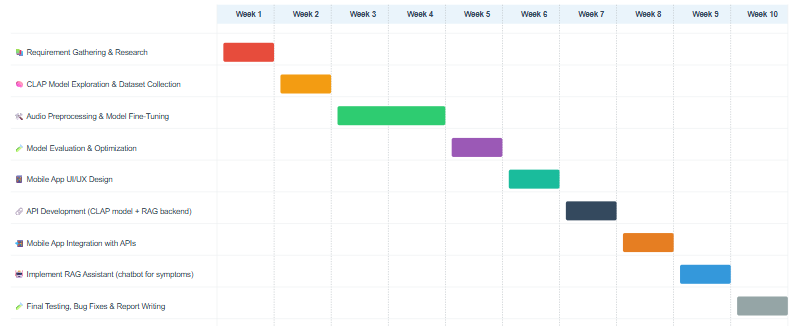
\includegraphics[width=\textwidth]{images/Gannt.png}
    \caption{Project timeline represented with a Gantt chart.}
    \label{fig:gantt-chart}
\end{figure}
\newpage

\setcounter{chapter}{2}  % Start from chapter 2
\setcounter{section}{0}
\chapter*{Chapter 2:\\ Business Understanding and Key Concepts}
% intro + 2.1 + 2.2

\section*{Introduction}
Respiratory diseases are among the leading causes of morbidity and mortality worldwide. Conditions such as asthma, pneumonia, bronchitis, and chronic obstructive pulmonary disease (COPD) often present with distinct acoustic signatures in lung sounds. Early and accurate detection of these anomalies can significantly improve clinical outcomes, reduce hospital admissions, and lower healthcare costs. Traditional auscultation with a stethoscope, though effective, is highly subjective and dependent on clinical expertise. This project leverages deep learning and multimodal processing to automate the classification of respiratory sounds using both audio and clinical metadata, aiming to support clinicians with an objective and reproducible decision-support tool.
\newpage

\section{Project Domain – Respiratory Anomalies}

\paragraph{2.1.1 Respiratory Anomalies and Their Significance\\}
Respiratory anomalies are abnormal sounds heard during lung auscultation, which are indicative of underlying pulmonary conditions. Common anomalies include:

\begin{itemize}
    \item \textbf{Wheezing:} A high-pitched, musical sound typically associated with narrowed airways and conditions such as asthma or COPD.
    \item \textbf{Crackles (Rales):} Discontinuous popping sounds heard during inhalation, often indicating fluid in the alveoli as seen in pneumonia or pulmonary fibrosis.
\end{itemize}

\paragraph{Importance of Early Detection in Healthcare\\}
Early diagnosis of respiratory diseases through anomaly detection can:

\begin{itemize}
    \item Enable timely medical intervention and prevent disease progression.
    \item Reduce the need for costly imaging or invasive diagnostic procedures.
    \item Facilitate remote diagnosis in telemedicine and resource-limited settings.
    \item Assist in large-scale screening, especially during pandemics or respiratory outbreaks.
\end{itemize}

This project's integration of both audio recordings and patient metadata (extracted from clinical PDF reports) aims to emulate real-world diagnostic scenarios where doctors rely on both auscultatory findings and patient history for diagnosis.

\section{Deep Learning Concepts}
\label{sec:deep-concepts}

\subsection*{Natural Language Processing}
\label{sssec:nlp}

Natural Language Processing (NLP) is a field of artificial intelligence that develops algorithms to enable machines to process, interpret, and generate human-like text. NLP empowers computers to perform language-related tasks traditionally requiring human intelligence, including Language translation, Sentiment analysis, Text classification, Information extraction


A key advancement in NLP has been the development of \textit{word embeddings} - numerical representations that capture semantic meaning and contextual relationships between words. These embeddings form the foundation for modern language understanding systems.



\subsection*{Word Embeddings}
\label{sssec:word-embeddings}

Word embeddings are vector representations of words. The challenge they aim to address is the ability to represent similar words—i.e., words that often appear in similar contexts—with similar vectors, where the vector directions also carry semantic meaning. 

While word vectors had been previously used in information retrieval, one of their most pivotal applications was their integration into neural networks. The need for word embeddings became evident when researchers began feeding words into Neural Networks (NNs).

Several encoding strategies were considered:

\begin{itemize}
    \item \textbf{Character-based representation:} Training a character-level model consumes a large portion of the network's capacity to simply learn valid word forms, potentially limiting its ability to learn higher-level features such as context or semantics.
    
    \item \textbf{Dictionary-based representation:}
    \begin{itemize}
        \item \textit{One-hot encoding:} Each word is represented as a vector of length $N$ (the vocabulary size) with all entries set to 0 except for a 1 in the position corresponding to that word. This approach does not encode similarity and leads to sparse and high-dimensional data, which is inefficient.
        
        \item \textit{Index-based encoding:} Assigning a unique integer to each word implies false assumptions—e.g., that adjacent indices mean semantic closeness.
    \end{itemize}
\end{itemize}

These limitations highlighted the need for richer numerical representations that reflect both word meaning and context. Additionally, words can have multiple meanings in different contexts, motivating dynamic or multi-context embeddings.

\subsubsection*{Popular Embedding Models}

\begin{itemize}
    \item \textbf{Word2Vec:} This model learns embeddings by predicting context words given a target word (Skip-Gram) or predicting a word from its context (Continuous Bag-of-Words, or CBOW). Word2Vec optimizes training speed and scalability through techniques like \textit{Negative Sampling}. It excels at capturing local context and performs well on tasks like word prediction.
    
    \item \textbf{GloVe (Global Vectors):} GloVe is an unsupervised learning algorithm that constructs a co-occurrence matrix capturing the frequency with which word pairs appear together in a corpus. It then factorizes this matrix to produce dense word vectors. GloVe captures both local and global context but may struggle with tasks involving polysemous words (words with multiple meanings).
\end{itemize}

\subsubsection*{Vector Analogies}

Word embeddings allow for interesting arithmetic operations that reveal semantic relationships. A well-known example illustrates this with gender analogies:

\begin{quote}
\centering
\texttt{vector("king") - vector("man") + vector("woman") $\approx$ vector("queen")}
\end{quote}

This vector analogy demonstrates that the learned embedding space encodes meaningful relationships such as gender differences, enabling analogical reasoning.

\begin{figure}[htbp]
  \centering
  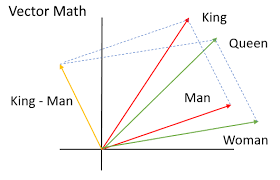
\includegraphics[width=0.5\textwidth]{images/Word Embedding Example.png}
  \caption*{\textbf{Figure 1:} The classical \textit{king - man + woman = queen} example of word embeddings.} % Starred version
  \label{fig:indexing-process-manual}
\end{figure}

Word embeddings are widely used in NLP tasks such as sentiment analysis, machine translation, and question answering. Interestingly, research has shown that source code exhibits similar co-occurrence patterns to natural language. As a result, vector representations of tokens in programming languages have also been explored using similar embedding techniques.

\subsection*{Audio Embeddings}
\label{sssec:audio-embeddings}

Audio embeddings are numerical representations of audio samples that capture essential characteristics and features of the sound. These embeddings are widely used in applications such as audio classification, music recommendation, and speech recognition. Essentially, an audio embedding transforms complex audio data into a fixed-size vector, making it easier for machine learning models to analyze and compare different audio samples. This compact vector encodes information such as pitch, rhythm, timbre, and other auditory features.

The process of generating audio embeddings typically involves several steps:

\begin{itemize}
    \item \textbf{Pre-processing:} The raw audio signal is first pre-processed. Common steps include noise reduction, normalization, and segmentation into smaller chunks or frames.
    
    \item \textbf{Feature extraction:} From the pre-processed audio, features are extracted using techniques such as:
    \begin{itemize}
        \item \textit{Short-Time Fourier Transform (STFT)}
        \item \textit{Mel-Frequency Cepstral Coefficients (MFCC)}
        \item \textit{Mel-spectrograms}
    \end{itemize}
    These methods help capture the frequency content of the audio over time, allowing models to encode meaningful auditory information.
    
    \item \textbf{Embedding generation:} Machine learning models such as Convolutional Neural Networks (CNNs) or Recurrent Neural Networks (RNNs) are applied to the extracted features to produce dense vector embeddings. 
\end{itemize}

For instance, CNNs may learn to recognize different instruments or environmental sounds, while RNNs can capture temporal patterns in speech or music. The resulting embedding is a fixed-size vector that summarizes the most relevant properties of the audio sample.

These audio embeddings are then used for downstream tasks such as clustering, retrieval, or classification, enabling systems to interpret and manipulate audio data effectively in various contexts.

\subsection*{Large Language Models}
\label{sssec:llms}

A language model is a statistical representation of a human language, capable of estimating the likelihood of word sequences based on the text data it was trained on.

In their most advanced form, \textit{Large Language Models} (LLMs) are a fusion of feedforward neural networks and transformers. LLMs are characterized by three major features:

\begin{itemize}
    \item \textbf{Scale:} LLMs are trained on extremely large datasets and have a vast number of parameters, often exceeding one billion.
    \item \textbf{General-purpose capabilities:} These models are capable of performing a wide range of tasks, including language generation, summarization, translation, question answering, and even solving mathematical problems.
    \item \textbf{Fine-tuning potential:} Although LLMs are trained on general data, they can be fine-tuned for specific tasks using much smaller, task-specific datasets.
\end{itemize}

LLMs leverage Deep Learning (DL) techniques—particularly the transformer architecture—to capture the complex dependencies and hierarchical structures present in natural language. Notable examples include \textit{GPT-3} (Generative Pre-trained Transformer 4) and \textit{Llama 3.2}.

The emergence of transformers has played a critical role in the development of LLMs, enabling them to understand and generate human-like text with high fluency and contextual awareness. Transformers are now the standard architecture underlying most modern LLMs.

\subsection*{Transformers}
\label{sssec:transformers}

Transformers are a Neural Network architecture that have revolutionized Natural Language Processing (NLP). Neural Networks are capable of analyzing vast amounts of data, including images, videos, text, and audio. Each data type is best suited for specific neural architectures; for instance, Convolutional Neural Networks (CNNs) are optimized for visual data.

CNNs simulate how the human brain processes visual information and are particularly powerful for tasks like object detection, facial recognition, and handwritten text recognition. However, for language-related tasks, CNNs were not the most effective.

To address this, Recurrent Neural Networks (RNNs) were developed for handling sequential data, as shown in Figure~\ref{fig:rnn_architecture}. RNNs could capture temporal dependencies and were widely used for language modeling tasks. However, they struggled with long-term dependencies due to issues like the vanishing and exploding gradient problems. This made them difficult to train and limited their ability to remember information across long sequences.

\begin{figure}[htbp]
  \centering
  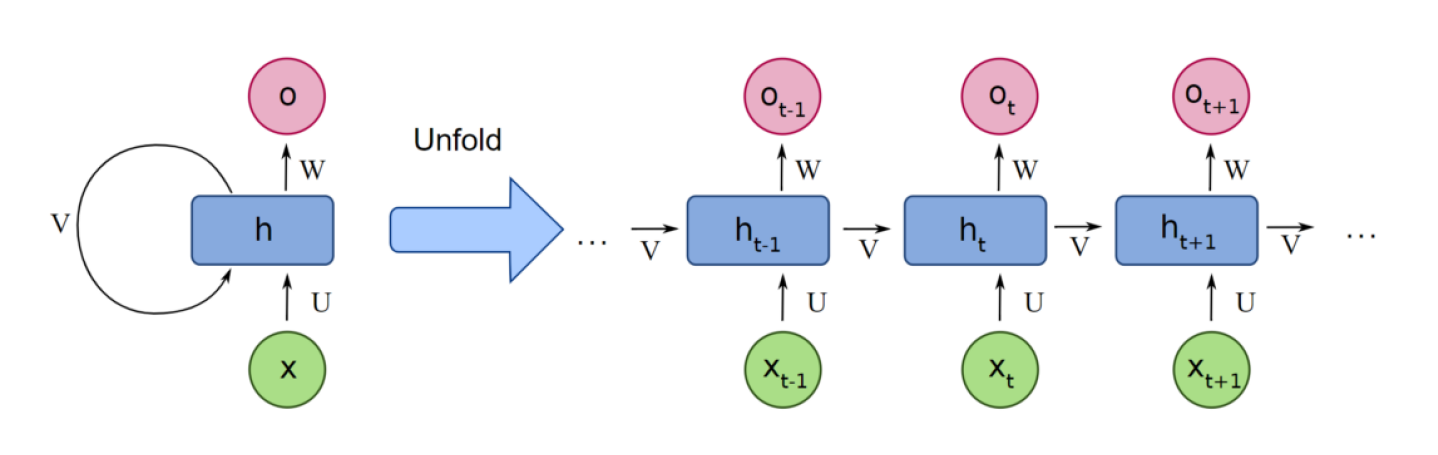
\includegraphics[width=1\textwidth]{images/RNN.png}
  \caption*{\textbf{Figure 1:} RNN Architecture} % Starred version
  \label{fig:rnn_architecture}
\end{figure}

In 2017, the introduction of Transformers by researchers from Google and the University of Toronto marked a significant breakthrough. Initially designed for translation tasks, the Transformer architecture has since become the standard for modern NLP models.

Unlike RNNs, Transformers can be easily parallelized, which allows for the training of extremely large models. The architecture of the Transformer is illustrated in Figure 2.

\begin{figure}[H]
  \centering
  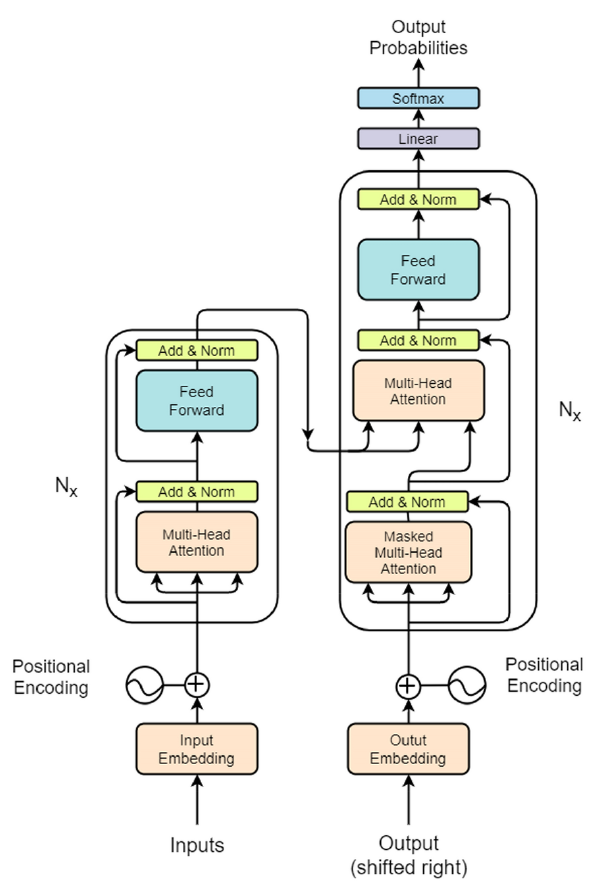
\includegraphics[width=0.55\textwidth]{images/Transformer Architecture.png}
  \caption*{\textbf{Figure 2:} Transformer Diagram from the original paper ``Attention is All You Need''} % Starred version
  \label{fig:transformer_architecture}
\end{figure}

Transformers are based on three key concepts:

\begin{itemize}
    \item \textbf{Positional Encodings:} Since Transformers do not process input sequences in order like RNNs, positional encodings are added to each word to preserve the sequence information. Originally, sinusoidal functions were used to generate these encodings, and the model learns to interpret them during training.

    \item \textbf{Attention:} Introduced in 2015, the attention mechanism assigns a contextual weight to each word in the input, allowing the model to focus on the most relevant parts of a sentence. This is not based solely on individual words, but on the entire context.

    \item \textbf{Self-Attention:} This is a special form of attention where the model considers the same input sequence to compute the relationships between its elements. Self-attention helps capture dependencies across the whole sequence simultaneously, ensuring that important information is retained throughout the process.
\end{itemize}

Not all Transformer models are the same. There are many architectural variations designed for specific tasks, such as BERT for masked language modeling, GPT for autoregressive generation, and T5 for text-to-text tasks. Despite these differences, they all share the same foundational principles of attention and positional encoding.

\subsection*{Retrieval-Augmented Generation (RAG)}

Retrieval-Augmented Generation (RAG) is a hybrid architecture that combines the strengths of retrieval-based and generative models. Instead of relying solely on pre-trained knowledge, RAG enhances a generative language model by incorporating external documents retrieved from a large corpus in real time.

The architecture consists of two main components:

\begin{itemize}
    \item \textbf{Retriever:} Fetches relevant documents or passages based on the input query, typically using dense or sparse retrieval methods.
    \item \textbf{Generator:} A language model that conditions its output on both the input query and the retrieved documents to generate accurate and informative responses.
\end{itemize}

RAG is particularly useful in knowledge-intensive tasks such as question answering and summarization, where grounding the output in factual information is crucial.


\subsection*{CLAP (Contrastive Language-Audio Pretraining)}

CLAP is a neural network model designed to learn joint representations of audio and natural language. By employing contrastive learning techniques, CLAP aligns audio signals with their corresponding textual descriptions in a shared embedding space. This approach enables the model to perform tasks such as zero-shot audio classification, retrieval, and captioning without the need for task-specific training.

The architecture of CLAP consists of two main components:

\begin{itemize}
    \item \textbf{Audio Encoder:} Processes audio inputs, typically using a SWIN Transformer, to extract meaningful features from log-Mel spectrograms.
    \item \textbf{Text Encoder:} Utilizes models like RoBERTa to convert textual descriptions into feature representations.
\end{itemize}

Both audio and text features are projected into a common latent space, allowing the model to measure similarity between audio clips and textual inputs effectively. This design facilitates various applications, including audio-text retrieval and zero-shot classification, by leveraging the semantic alignment between modalities.

\section{Mobile Development Concepts}
\label{sec:mobile_concepts}

Mobile development refers to the design and creation of software applications intended to operate on mobile devices such as smartphones and tablets. In the context of this project, mobile development serves as the foundation for the user-facing component of the system, enabling users to interact with diagnostic features, access results, and consult the AI assistant. This section introduces the key mobile development concepts relevant to the architecture used in this work.

\subsubsection*{Cross-Platform Development}

Cross-platform development is a software development approach that allows a single application codebase to be deployed on multiple operating systems, most notably Android and iOS. This reduces redundancy and development effort while maintaining consistency in functionality and design. It is especially beneficial in healthcare applications, where uniform user experience and rapid iteration are critical.

\subsubsection*{Modular Mobile Architecture}

A modular architecture divides the application into independent functional units, such as user interface components, business logic, and data services. This separation of concerns improves scalability, testability, and long-term maintainability. It also supports incremental feature integration—particularly important in complex systems like diagnostic platforms.

\subsubsection*{User-Centered Design in Health Applications}

Mobile health applications must prioritize accessibility, clarity, and ease of use. User-centered design (UCD) involves tailoring the interface to user needs, using intuitive navigation, medically neutral colors, and readable typography. These design principles are especially important in applications intended for patients, where cognitive load and clarity directly impact usability.

\subsubsection*{Data Privacy and Security Principles}

Mobile applications that handle health-related data must comply with strict privacy and security guidelines. Core concepts include local data encryption, secure authentication flows, permission-based access to device hardware (e.g., microphone), and encrypted communication channels. These safeguards help ensure that personal health information is protected throughout the diagnostic process.

\subsubsection*{Real-Time and Asynchronous Interaction}

Many mobile applications rely on real-time feedback and asynchronous operations—such as sending diagnostic data to a server and waiting for results. Concepts such as event-driven programming, state management, and asynchronous networking are fundamental to building responsive, interactive experiences without blocking the user interface.

\subsubsection*{Summary}

This section introduced the theoretical foundations of mobile development as they apply to healthcare systems. Concepts such as cross-platform development, modular architecture, security, and user-centered design provide the groundwork for implementing reliable and accessible diagnostic tools on mobile platforms. These principles informed the design decisions detailed later in the implementation chapter.

\section*{Conclusion}
\addcontentsline{toc}{section}{Conclusion}

\label{sec:chapter2_conclusion}

This chapter introduced the key domains that underpin the design of our AI-powered respiratory diagnosis system. These domains—medical anomalies, deep learning, and mobile development—serve as the conceptual foundation for the project's implementation.

First, we explored the nature of respiratory anomalies and their clinical significance, highlighting sounds such as wheezing, crackles, and stridor. These sounds provide early indicators of diseases like asthma, pneumonia, and COPD. Understanding their acoustic characteristics is essential for developing diagnostic algorithms that can detect them automatically.

Second, we reviewed core deep learning concepts, with a focus on audio classification using models such as CLAP, as well as the use of large language models (LLMs) for natural language understanding. These AI tools enable the system to both analyze user-recorded audio and provide conversational explanations and guidance through the integrated assistant.

Finally, we presented key mobile development concepts relevant to our implementation. Cross-platform development, modular architecture, responsive design, and data privacy principles ensure that the system remains accessible, secure, and user-friendly across devices. These concepts support the delivery of accurate, real-time diagnostics directly through a mobile interface.

Together, these foundations—clinical, algorithmic, and technical—set the stage for the practical implementation of our system, detailed in the chapters that follow.


\newpage

\setcounter{chapter}{3}
\setcounter{section}{0}
\chapter*{Chapter 3 :\\ State-of-the-art and related work}
\paragraph{Introduction\\}
Respiratory sound classification is a key component in the development of AI-assisted tools for pulmonary disease screening. This section reviews existing methodologies used for analyzing lung sounds, outlines performance on a common benchmark dataset, and identifies key limitations in current approaches. We conclude by presenting our contribution, which addresses these gaps through a multimodal, deployment-ready framework.

\newpage

\paragraph{3.1 Overview of Respiratory Sound Classification\\}
Research in respiratory disease detection using lung auscultation audio has expanded rapidly, with significant emphasis on early, non-invasive diagnosis. Classical approaches have relied on signal processing techniques like MFCCs and wavelets combined with shallow classifiers (e.g., SVMs, Random Forests). More recent studies employ deep learning — particularly convolutional and recurrent architectures — trained directly on spectrograms or raw waveforms.

\paragraph{3.2 The ICBHI Dataset and Prior Work\\}
The ICBHI 2017 Respiratory Sound Database is a benchmark dataset containing over 5.5 hours of annotated lung sounds from 126 patients, labeled for the presence of crackles, wheezes, both, or normal \cite{rocha2017open}. Several studies have evaluated models on this dataset with a focus on binary or multi-class classification.

\paragraph{3.3 Comparative Performance on ICBHI Dataset\\}
\begin{table}[h!]
\centering
\small
\renewcommand{\arraystretch}{1.2}
\begin{tabular}{|p{3.2cm}|p{2.2cm}|p{1.5cm}|p{2.2cm}|p{4cm}|}
\hline
\textbf{Model} & \textbf{Input} & \textbf{Classes} & \textbf{F1 / Acc.} & \textbf{Notes} \\
\hline
Perna et al. (2019) \cite{perna2019} & MFCC + CNN & 3 & 85.3\% (Acc.) & Spectrogram-based CNN model \\
Demir et al. (2021) \cite{demir2021} & ResNet + MFCC & 3 & 88.7\% (F1) & Ensemble of CNNs trained on MFCC features \\
Ibrahim et al. (2020) \cite{ibrahim2020} & BiLSTM & 3 & 84.5\% (F1) & Temporal sequence modeling using recurrent layers \\
Aygun et al. (2022) \cite{aygun2022} & EfficientNet + SpecAugment & 3 & 90.2\% (Acc.) & CNNs with spectrogram augmentation techniques \\
\hline
\end{tabular}
\caption*{Table 3.2.1: Comparison of respiratory sound classification models on the ICBHI dataset.}
\label{tab:icbhi_comparison}
\end{table}
\vspace{0.5em}
\textit{Note: Differences in dataset splits, class definitions, and preprocessing methods make direct comparison approximate.}

\paragraph{3.4 Limitations in Existing Approaches\\}
Despite high reported accuracies, most existing studies suffer from:
\begin{itemize}
    \item \textbf{Modality Limitation:} Only use audio data; no use of patient context.
    \item \textbf{Device Heterogeneity:} Include both stethoscope and microphone recordings, reducing consistency.
    \item \textbf{Lack of Deployment Focus:} No exploration of real-time, user-facing APIs or interfaces.
\end{itemize}

\paragraph{3.5 Our Contribution and Innovation\\}
Our work advances the field with:
\begin{itemize}
    \item \textbf{Microphone-only Data:} More relevant to smartphone-based real-world recordings.
    \item \textbf{Textual Metadata Integration:} Clinical descriptions extracted from PDFs enhance context.
    \item \textbf{Multimodal CLAP Embedding:} Fuses audio and text for richer, patient-aware predictions.
    \item \textbf{End-to-End Deployment:} A FastAPI server enables immediate, interactive use for real scenarios.
\end{itemize}

\paragraph{Conclusion\\}
This section has explored the state of respiratory sound classification, highlighting both the strengths and blind spots of recent methods. While performance metrics on the ICBHI dataset are promising, most models overlook practical constraints such as recording device variation and lack of contextual patient data. Our multimodal, deployment-ready system directly addresses these issues, positioning it for real-world use in accessible respiratory diagnostics.



\setcounter{chapter}{4}
\chapter*{Chapter 4 :\\ Respiratory Sound Classification}
\input{Chapter4/4.1Business Understanding}
\section*{4.2 Data Understanding}

\paragraph{4.2.1 Data Sources \\}
The primary dataset used for training the model is the \textbf{ICBHI 2017 Respiratory Sound Database}, which includes:
\begin{itemize}
    \item \textbf{Audio recordings} of lung sounds collected from 126 patients using an electronic stethoscope.
    \item \textbf{Metadata files}, such as demographic information and clinical diagnoses.
    \item \textbf{Segmentation annotations} indicating labeled intervals of respiratory events (inspiration, expiration).
\end{itemize}

\paragraph{4.2.2 Loaded Data\\}
Three key components were extracted:
\begin{enumerate}
    \item \textbf{Diagnosis Labels:} A CSV file (\texttt{patient\_diagnosis.csv}) mapping patient IDs to their respiratory condition (e.g., asthma, COPD, pneumonia).
    \item \textbf{Demographic Metadata:} A text file containing age, sex, BMI, and child-specific attributes like height and weight.
    \item \textbf{Audio Files:} Multiple WAV files per patient, capturing respiratory cycles in varying environments and conditions.
\end{enumerate}

\paragraph{4.2.3 Exploratory Analysis\\}
The following steps were conducted to better understand the data:
\begin{itemize}
    \item Inspected class distribution to identify imbalance (e.g., overrepresentation of "healthy" vs. "COPD").
    \item Visualized audio signal characteristics such as waveform length, sampling rate consistency, and signal-to-noise ratio.
    \item Merged demographic and diagnosis data by patient ID to facilitate multimodal embedding.
    \item Generated descriptive sentences per patient from structured metadata, such as:
    \textit{"Patient 101 is a 65-year-old male. The adult has a BMI of 27.3 kg/m²."}
\end{itemize}

\paragraph{4.2.4 Challenges Identified\\}
\begin{itemize}
    \item \textbf{Missing Data:} Some entries lack age, BMI, or diagnosis labels, requiring filtering or imputation.
    \item \textbf{Class Imbalance:} Certain respiratory conditions are underrepresented, potentially biasing the classifier.
    \item \textbf{Variable Audio Lengths:} Recording durations vary significantly, requiring padding or trimming during preprocessing.
    \item \textbf{Data Heterogeneity:} Audio captured in uncontrolled environments introduces noise and inconsistency.
\end{itemize}

\paragraph{Summary \\}
The dataset provides a rich combination of audio and clinical metadata, which is essential for multimodal learning. By using CLAP to embed both the auscultation sounds and textual descriptions, the project exploits this diversity to improve classification performance. A thorough understanding of the dataset’s structure and limitations guided preprocessing and model design choices.


\section{Data Preparation}

\subsection*{Overview}
To enable the use of the CLAP (Contrastive Language-Audio Pretraining) model, both audio signals and textual descriptions were preprocessed and aligned into a format suitable for joint embedding. Data preparation involved several key stages: cleaning, transformation, feature generation, and multimodal input construction.

\subsection{Audio Preprocessing}
\begin{itemize}
    \item \textbf{Loading:} WAV audio files were loaded using \texttt{torchaudio} with consistent settings across all samples.
    \item \textbf{Resampling:} All audio signals were resampled to 48\,kHz to match the input requirements of the CLAP model.
    \item \textbf{Normalization:} Amplitude normalization was applied to reduce variability in recording loudness.
    \item \textbf{Device Filtering:} Only audio recorded using a microphone device was retained; recordings captured via stethoscope or user-recorded samples were excluded to ensure consistency and realistic ambient conditions.
\end{itemize}

\subsection{Text Preprocessing}
\begin{itemize}
    \item \textbf{Demographic Metadata Integration:} Patient age, sex, and physical metrics were combined into a coherent textual description.
    \item \textbf{Description Generation:} A custom function generated natural language sentences, e.g., \textit{"Patient 103 is a 7-year-old female child weighing 22 kg and measuring 120 cm in height."}
    \item \textbf{Tokenization:} Descriptions were tokenized using the CLAP processor to match the format of its language encoder.
    \item \textbf{Missing Value Handling:} Patients missing critical metadata fields were assigned defaults.
\end{itemize}

\subsection{Multimodal Pair Construction}
Each input sample consisted of a synchronized multimodal pair:
\begin{enumerate}
    \item A preprocessed 5-second audio tensor representing a single breathing cycle.
    \item A text description specific to the patient from whom the audio was collected.
\end{enumerate}
These were fed into the CLAP model to generate aligned audio-text embeddings in a shared latent space.

\subsection{Label Encoding}
\begin{itemize}
    \item Respiratory condition labels (e.g., crackles, wheezes, normal) were derived from expert annotations per breathing cycle.
    \item Labels were encoded using \texttt{LabelEncoder} from \texttt{scikit-learn} to obtain numerical class indices.
    \item Ambiguous or unlabeled cycles were excluded to avoid introducing noise in the training process.
\end{itemize}

\subsection{Dataset Splitting}
\begin{itemize}
    \item An official dataset split provided by the dataset curators was used to separate training and test sets.
    \item This ensured reproducibility and comparability with prior work.
    \item Patient-level disjointness was maintained: no subject appeared in both training and test sets, preventing data leakage.
\end{itemize}

\subsection*{Summary}
The preprocessing pipeline standardized and aligned audio and text inputs for CLAP-based embedding. Filtering by recording device, adherence to the official train/test split, and careful label and segmentation handling ensured high-quality inputs for downstream classification.

\break
\section{Modeling}

\paragraph{Overview}
The core modeling strategy involves using the CLAP (Contrastive Language-Audio Pretraining) model to transform heterogeneous input data — audio signals and textual patient metadata — into a unified latent representation. These embeddings are then passed through a custom multi-layer neural network for classification.

\begin{figure}[H]
    \centering
    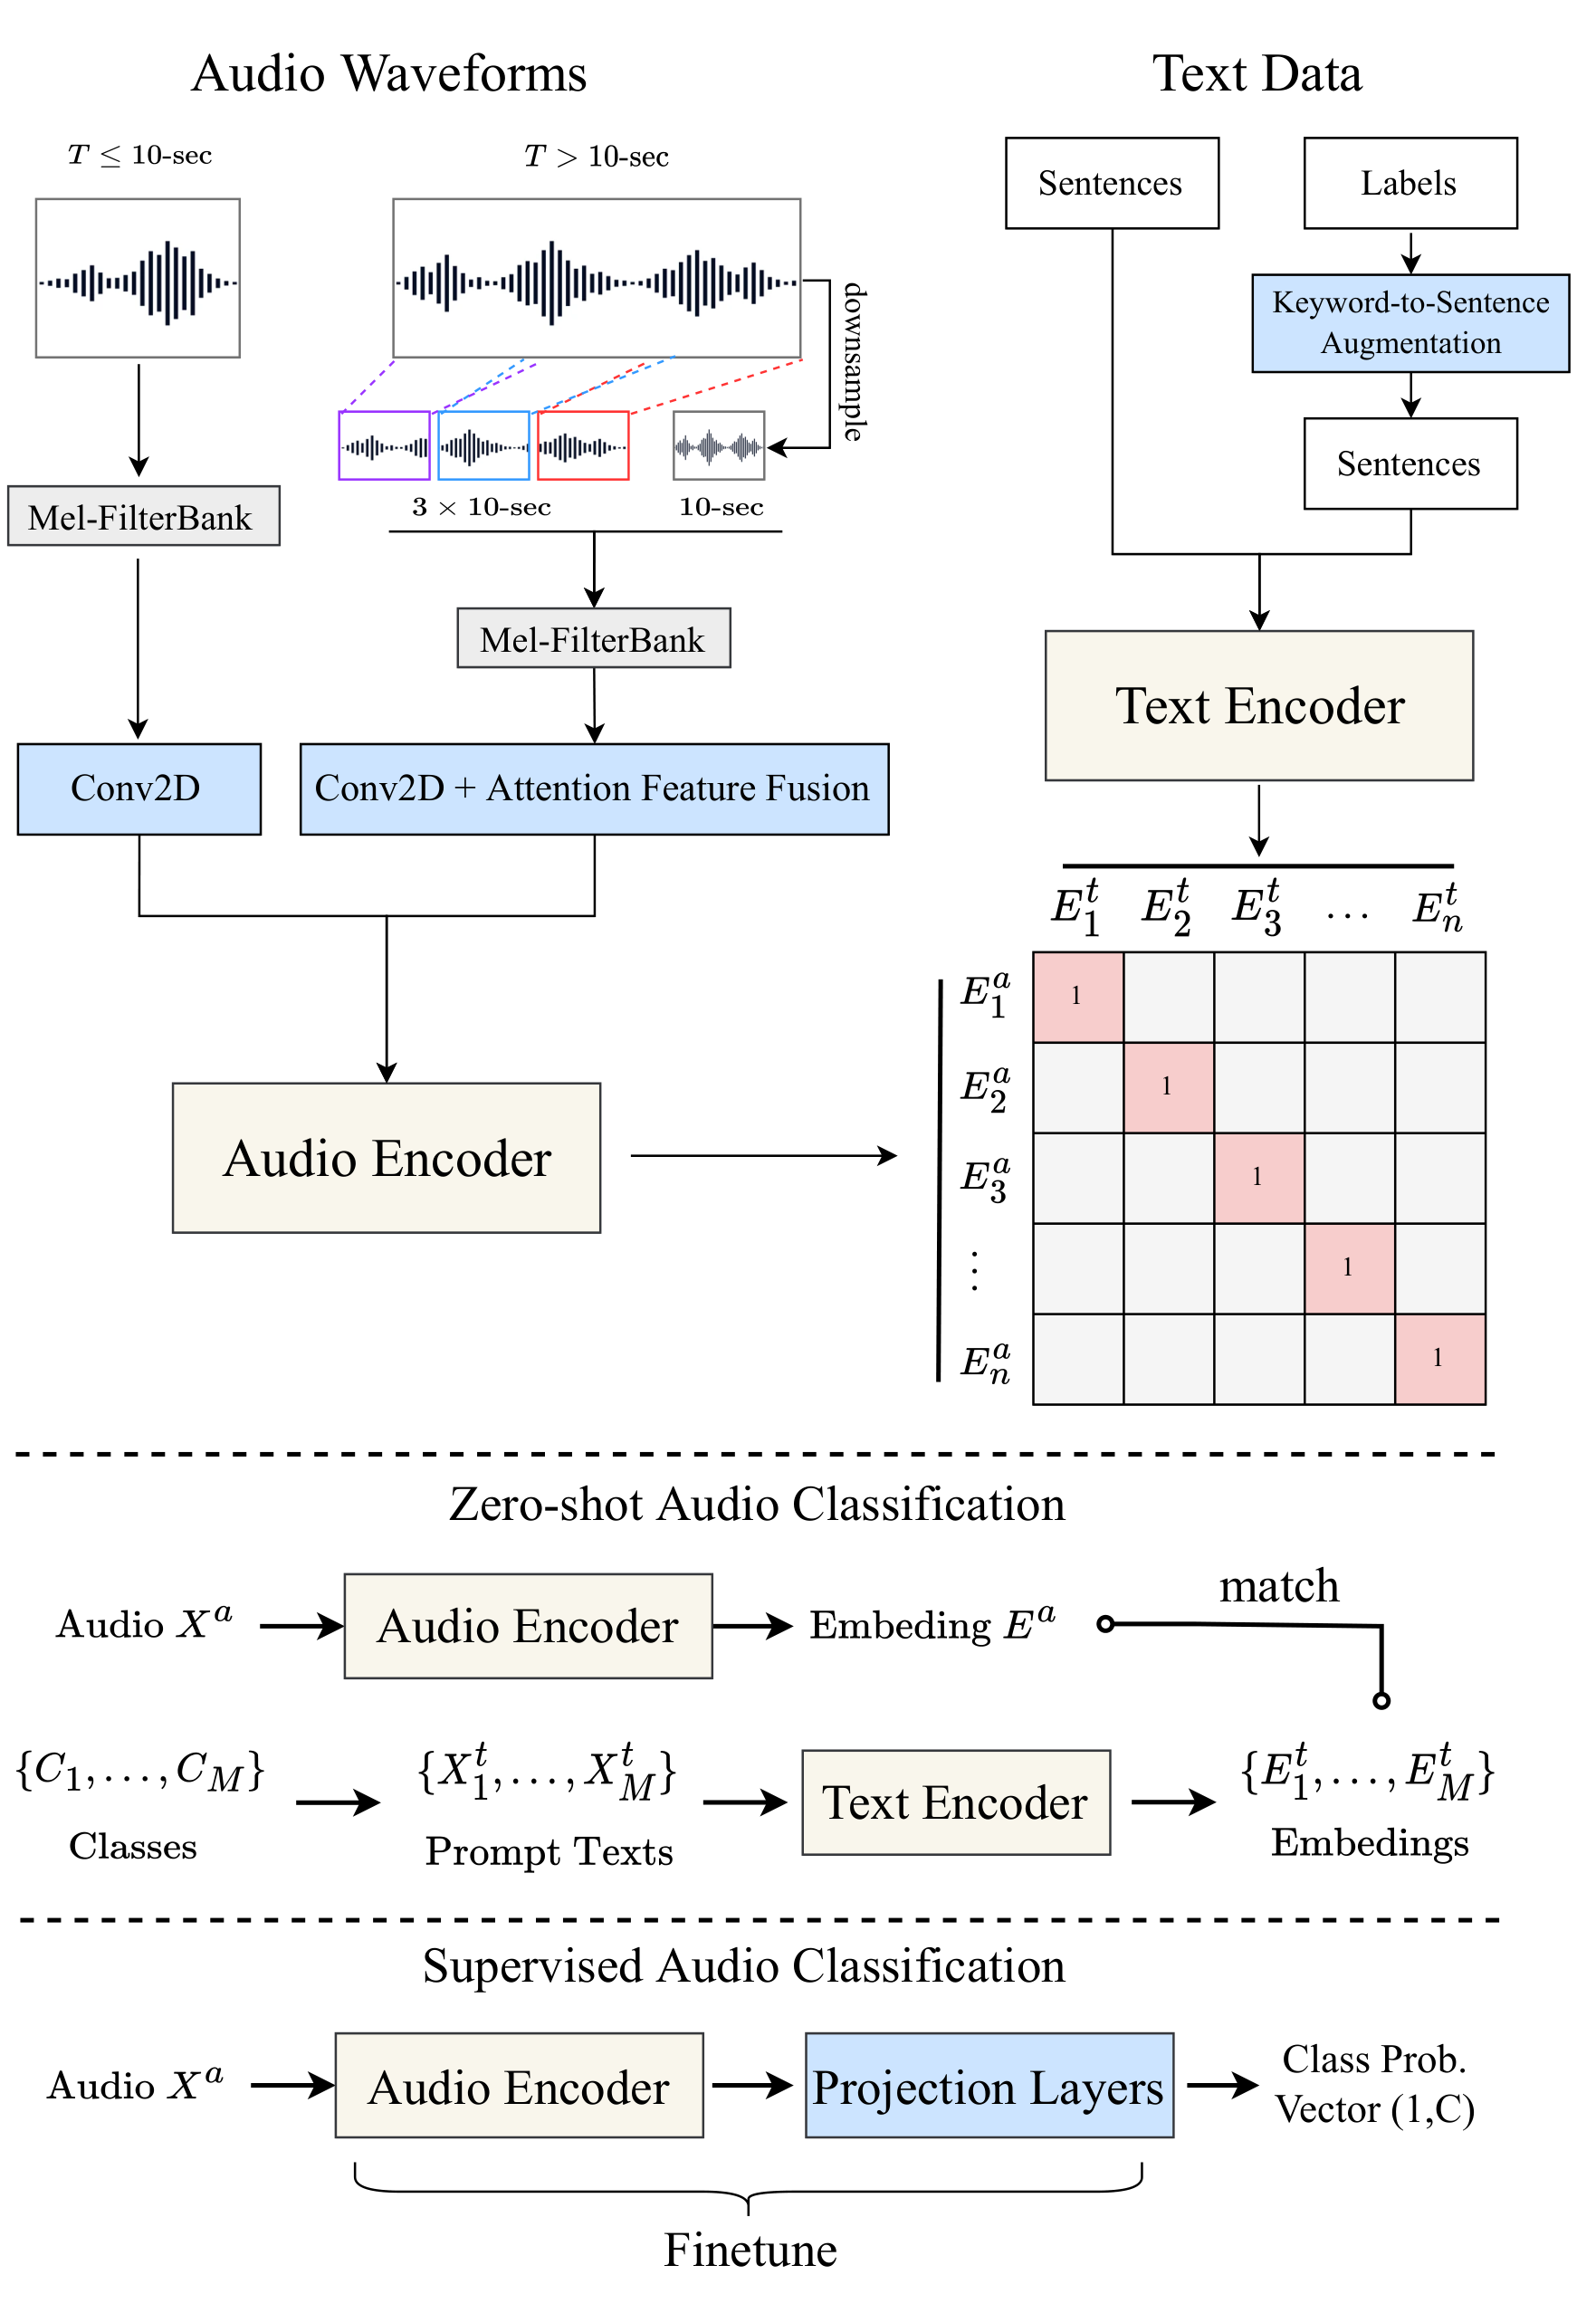
\includegraphics[width=0.6\textwidth]{Chapter4/audioclip-arch.png}
    \caption{CLAP model architecture used for embedding audio and text.}
    \label{fig:clap-model}
\end{figure}

\paragraph{CLAP: Multimodal Embedding Model}
CLAP is a transformer-based model trained to align audio and text modalities in a shared embedding space. It consists of two separate encoders:
\begin{itemize}
    \item \textbf{Audio Encoder:} Processes raw waveforms into feature embeddings using convolutional layers followed by transformers.
    \item \textbf{Text Encoder:} A transformer-based language model (similar to BERT) that embeds textual patient metadata.
\end{itemize}

The output of each encoder is a fixed-length vector, and CLAP is pretrained using contrastive learning to pull semantically aligned audio-text pairs closer in the embedding space.

\paragraph{Embedding Generation for Classification}
For this task:
\begin{itemize}
    \item Each breathing cycle was segmented from the audio and paired with patient text data.
    \item These inputs were passed through the CLAP model to generate audio and text embeddings.
    \item The embeddings were concatenated into a single feature vector.
    \item This fused embedding was used as input to a downstream neural classifier.
\end{itemize}

\paragraph{Classifier Architecture}
The classifier is a deep feedforward neural network with batch normalization, dropout regularization, and ReLU activations:
\begin{itemize}
    \item \textbf{Input:} Fused embedding vector of dimension $d$ (audio + text).
    \item \textbf{Layer 1:} Linear($d$, 512) $\rightarrow$ BatchNorm $\rightarrow$ ReLU $\rightarrow$ Dropout(0.5)
    \item \textbf{Layer 2:} Linear(512, 256) $\rightarrow$ BatchNorm $\rightarrow$ ReLU
    \item \textbf{Layer 3:} Linear(256, 64) $\rightarrow$ BatchNorm $\rightarrow$ ReLU
    \item \textbf{Output:} Linear(64, 3) $\rightarrow$ Softmax over respiratory classes (normal, crackles, wheezes)
\end{itemize}

\paragraph{Training Procedure}
\begin{itemize}
    \item \textbf{Loss Function:} Cross-entropy loss for multi-class classification.
    \item \textbf{Optimizer:} AdamW with initial learning rate of $1 \times 10^{-3}$ and weight decay of $1 \times 10^{-3}$.
    \item \textbf{Learning Rate Scheduler:} CosineAnnealingLR with $T_{\text{max}} = 10$.
    \item \textbf{Epochs:} Trained for 100 epochs with early stopping based on validation loss.
    \item \textbf{Batch Size:} Mini-batches of 32 samples for efficient GPU usage.
    \item \textbf{Fine-tuning Strategy:} CLAP weights were frozen during classifier training to preserve pretrained semantics and reduce training time.
\end{itemize}

\paragraph{Model Variants and Experiments}
Different modeling choices were explored to optimize performance:
\begin{itemize}
    \item \textbf{Fusion Strategy:} Simple concatenation of audio and text embeddings.
    \item \textbf{Embedding Size:} Tested with different encoder output dimensions.
    \item \textbf{Depth and Width of Classifier:} Adjusting hidden layer sizes and number of layers.
    \item \textbf{Freezing vs. Fine-tuning CLAP:} Partial fine-tuning yielded marginal improvements but increased training time.
\end{itemize}

\paragraph{Summary}
The modeling pipeline effectively combines audio and textual modalities through CLAP embeddings. A deep, regularized classifier leverages these representations for accurate respiratory sound classification. This architecture strikes a balance between expressiveness and efficiency, supporting real-time inference and deployment on modest hardware.

\break
\section{Evaluation}

\subsection*{Overview}
The model was evaluated on a held-out test set of 1,732 breathing cycles. Each sample included a fused CLAP embedding of audio and patient metadata. The classification targets were \texttt{normal}, \texttt{crackles}, and \texttt{wheezes}.

\begin{figure}[htbp]
    \centering
    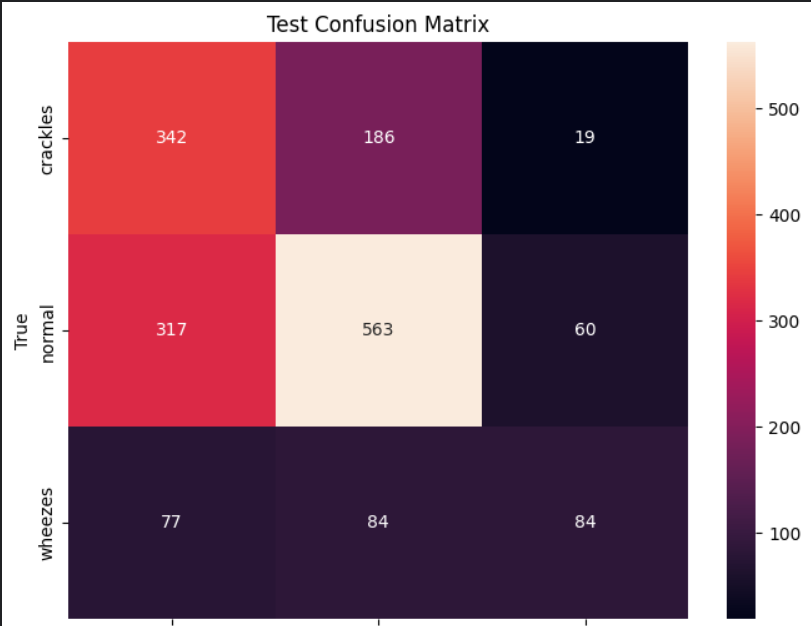
\includegraphics[width=0.7\linewidth]{Chapter4/pic.png}
    \caption{Test confusion matrix for respiratory sound classification.}
    \label{fig:confusion-matrix}
\end{figure}

\subsection{Performance Metrics}
\begin{itemize}
    \item \textbf{Accuracy:} 57.10\%
    \item \textbf{Macro F1-score:} 0.53
    \item \textbf{Weighted F1-score:} 0.57
    \item \textbf{Macro Precision:} 0.55
    \item \textbf{Macro Recall:} 0.52
\end{itemize}

\begin{table}[htbp]
\centering
\begin{tabular}{|l|c|c|c|c|}
\hline
\textbf{Class} & \textbf{Precision} & \textbf{Recall (Sensitivity)} & \textbf{F1-score} & \textbf{Support} \\
\hline
Crackles & 0.46 & 0.63 & 0.53 & 547 \\
Normal   & 0.68 & 0.60 & 0.64 & 940 \\
Wheezes  & 0.52 & 0.34 & 0.41 & 245 \\
\hline
\end{tabular}
\caption{Class-wise classification report.}
\end{table}

\subsection{Sensitivity and Specificity}
\begin{itemize}
    \item \textbf{Sensitivity (Recall):}
    \begin{itemize}
        \item Crackles: 0.625
        \item Normal: 0.599
        \item Wheezes: 0.343
        \item \textbf{Average:} 0.392
    \end{itemize}
    
    \item \textbf{Specificity:}
    \begin{itemize}
        \item Crackles: 0.668
        \item Normal: 0.659
        \item Wheezes: 0.947
        \item \textbf{Average:} 0.568
    \end{itemize}
\end{itemize}

\subsection{Observations}
\begin{itemize}
    \item The model performs best on the \texttt{normal} class, with an F1-score of 0.64.
    \item \texttt{Wheezes} are the hardest to classify (F1-score: 0.41), due to fewer examples and overlapping acoustic patterns with crackles.
    \item Specificity is highest for the \texttt{wheezes} class, indicating few false positives.
\end{itemize}

\subsection*{Summary}
The CLAP-based classifier shows promising overall accuracy and solid recall for crackles and normal sounds. Its lower sensitivity for wheezes suggests room for improvement through better balancing, augmentation, or fine-tuning the audio encoder. Still, the model maintains interpretability and scalability, aligning with the clinical goals of the system.

\section{Deployment (Model Serving)}

\paragraph{4.6.1 Overview\\}
To enable real-time inference, the trained multimodal CLAP-based classifier was deployed using a FastAPI web server. This server exposes a RESTful endpoint allowing users to upload a WAV audio file along with a patient information file in PDF format. The server extracts text from the PDF and combines it with the audio input to produce a diagnostic prediction.

\paragraph{4.6.2 File Structure\\}
The deployment folder contains the following core components:

\begin{itemize}
    \item \texttt{main.py} – FastAPI application containing preprocessing, inference, and routing logic.
    \item \texttt{model.pt} – Trained PyTorch classifier model weights.
    \item \texttt{label\_encoder.pkl} – Serialized \texttt{LabelEncoder} used to decode class indices into labels.
    \item \texttt{requirements.txt} – Specifies required Python libraries including \texttt{torch}, \texttt{transformers}, \texttt{PyMuPDF}, and \texttt{fastapi}.
    \item \texttt{Dockerfile} – Enables containerization of the app for consistent and scalable deployment.
\end{itemize}

\paragraph{4.6.3 API Endpoints\\}
Two endpoints are exposed:
\begin{itemize}
    \item \texttt{GET /} – Basic health check returning a simple greeting.
    \item \texttt{POST /predict} – Accepts:
    \begin{itemize}
        \item A WAV audio file.
        \item A PDF file containing patient information (e.g., age, sex, symptoms).
    \end{itemize}
    and returns a JSON response containing the predicted diagnostic label.
\end{itemize}

\paragraph{4.6.4 Processing Pipeline\\}
Upon receiving a request:
\begin{enumerate}
    \item The audio file is validated, loaded, resampled to 48\,kHz, converted to mono, and trimmed to a maximum of 8 seconds.
    \item The PDF file is parsed using \texttt{PyMuPDF} (\texttt{fitz}) to extract text-based metadata (e.g., "Patient is Male 36 , with BMI...").
    \item Audio and extracted text are processed using the CLAP processor to generate embeddings.
    \item Embeddings are passed to the trained classifier to generate class probabilities.
    \item The most probable class is decoded using \texttt{LabelEncoder} and returned.
\end{enumerate}

\paragraph{4.6.5 Robustness and Error Handling\\}
The API includes robust validation and fallback strategies:
\begin{itemize}
    \item Rejects non-WAV or non-PDF inputs.
    \item Handles corrupted or overly long audio clips.
    \item Gracefully processes empty or unreadable PDFs.
    \item Returns descriptive error messages and HTTP status codes for all edge cases.
\end{itemize}

\section*{4.7 Conclusion}
This section outlined the full CRISP-DM pipeline used to develop a multimodal respiratory sound classifier. By combining lung audio with patient metadata extracted from PDFs, the system leveraged CLAP embeddings for accurate, context-aware predictions. The final model was deployed using FastAPI, enabling real-time and scalable inference suitable for clinical settings.



\chapter{LLM-Based AI Assistant (RAG)} % This will automatically be Chapter 5
\label{chap:llm-rag}

\section*{Introduction}
This chapter explores the development of an intelligent assistant designed to support users with questions related to respiratory health. By combining language understanding with access to trusted medical information, the assistant aims to deliver clear, helpful, and relevant responses in real time. Our focus is on creating a system that is not only powerful but also accessible and responsible.

In the following sections, we walk through the key stages of building this assistant—from understanding the problem and preparing the data, to designing the system, evaluating its performance, and deploying it for real-world use.
\pagebreak  % Forces a new page



\section{Business Understanding} % Will auto-number as 5.1
% 5.1 Business Understanding.tex
\label{subsec:business-understanding}

The AI assistant, built using a Large Language Model (LLM) enhanced with Retrieval-Augmented Generation (RAG), is designed to provide users with accurate, contextual information about respiratory symptoms and diseases through natural language interaction. This tool complements the audio classification system by enabling users to ask questions and receive clear explanations and guidance related to their respiratory health.

\subsection*{Project Goals}
\begin{itemize}
    \item \textbf{Deliver Clear Medical Information:} Provide understandable explanations about respiratory anomalies such as wheezing and crackles detected by the system.
    
    \item \textbf{Support Decision-Making:} Assist both patients and doctors in interpreting symptoms and accessing relevant medical knowledge to make better-informed decisions.
    
    \item \textbf{Enhance Accessibility:} Offer users immediate and easy access to reliable respiratory health information without the need for expert presence.
    
    \item \textbf{Encourage User Engagement:} Foster continuous interaction by allowing users to ask follow-up questions and explore related health topics.
    
    \item \textbf{Integrate Seamlessly:} Work alongside the audio classification module to create a comprehensive and user-friendly respiratory health platform.
\end{itemize}

\subsection*{Challenges and Constraints}
\begin{itemize}
    \item \textbf{Medical Accuracy:} Ensure the assistant provides reliable and clinically sound responses to avoid misinformation.
    
    \item \textbf{Responsiveness:} Maintain fast and natural conversational interactions to improve user experience.
    
    \item \textbf{Scope Limitation:} Focus the assistant strictly on respiratory health information, not on clinical diagnosis or treatment.
\end{itemize}
\section{Data Understanding} % Will auto-number as 5.2
\label{sec:data-understanding}

To build an effective Retrieval-Augmented Generation (RAG) system, a high-quality and diverse knowledge base is essential. This phase focuses on understanding the types and characteristics of the data used to populate the assistant's knowledge base.

\subsection*{Data Collection Strategy}
To ensure the reliability and medical accuracy of the information, we performed targeted data scraping from trusted, verified medical sources:

\begin{itemize}
    \item \textbf{World Health Organization (WHO):} For global health guidelines and comprehensive information on respiratory conditions.
    
    \item \textbf{National Institutes of Health (NIH):} For research-based medical literature and symptom explanations.
    
    \item \textbf{Centers for Disease Control and Prevention (CDC):} For public health data, prevention guidelines, and symptom overviews.
\end{itemize}

In addition to these sources, we conducted extensive research to gather:

\begin{itemize}
    \item \textbf{Frequently Asked Questions (FAQs):} Common patient questions about respiratory diseases like asthma, bronchitis, pneumonia, COPD, etc.
    
    \item \textbf{Patient Education Content:} Short and accessible explanations to ensure the assistant can respond to both technical and non-technical queries.
\end{itemize}

\subsection*{Data Types}
\begin{itemize}
    \item \textbf{Unstructured Text:} Medical articles, clinical summaries, FAQs.
    
    \item \textbf{Semi-Structured Text:} Bullet points, Q\&A-style content from FAQs and health portals.
\end{itemize}

\subsection*{Data Coverage and Goals}
\begin{itemize}
    \item Ensure comprehensive coverage of the most common respiratory diseases, including symptoms, causes, treatment options, and prevention.
    
    \item Include both clinical terms (e.g., ``dyspnea'', ``rales'') and layperson vocabulary (e.g., ``shortness of breath'', ``crackles when breathing'') to accommodate diverse users.
    
    \item Capture a wide range of user intents: symptom explanation, general disease information, treatment advice (non-prescriptive), etc.
\end{itemize}
\section{Data Preparation} % Will auto-number as 5.3
\label{sec:data-preparation}

Once the raw data was collected from trusted sources, it had to be cleaned, standardized, and transformed into a format suitable for both retrieval and generation. This phase shown in the Figure 5.3.1 plays a crucial role in ensuring the quality and efficiency of the RAG pipeline.

\subsection{Cleaning and Filtering}
\label{subsec:cleaning-filtering}

The raw textual data extracted from sources like WHO and CDC websites often contained a mix of useful content and noise. A cleaning pipeline was applied to ensure only relevant and high-quality information was retained.

\begin{itemize}
    \item \textbf{Structural Cleaning:} HTML content was parsed and converted into plain text while preserving logical sections (e.g., paragraphs, headers). This ensured the data remained well-structured for further processing.
    
    \item \textbf{Removal of Irrelevant Elements:} Common non-informative parts such as headers, footers, ads, navigation menus, and update timestamps were removed using pattern-matching and HTML parsing.
    
    \item \textbf{Redundancy Elimination:} Duplicate or repetitive information—like repeated titles or boilerplate disclaimers—was identified and removed. When similar content appeared multiple times, the most complete or contextually rich version was kept.
\end{itemize}

This process significantly improved the clarity and usefulness of the final dataset used in the RAG pipeline.

\subsection{Chunking}
\label{subsec:chunking}

Once the data was cleaned and filtered, the next crucial step involved splitting the text into coherent and manageable segments, a process known as chunking. This step is essential for the retrieval phase of the RAG (Retrieval-Augmented Generation) system because it enables the model to work with smaller, more focused passages instead of entire articles.

We applied a fixed-length token chunking strategy, where the textual content was segmented into chunks of 800 tokens each. To maintain contextual continuity across chunks and ensure that important information was not cut off at the edges, we used a sliding window approach with an overlap of 80 tokens between consecutive chunks. This overlapping approach allowed us to preserve the flow of ideas, especially when key information spanned across chunk boundaries.

Choosing 800 tokens as the chunk size provided a balance between depth of context and computational efficiency. Each chunk was large enough to capture meaningful information, such as a complete explanation of a symptom or a treatment recommendation, while still being short enough to work efficiently within the input limits of the language model.

These context-rich chunks formed the basic units for the embedding and retrieval process that powers the RAG system.

\subsection{Metadata Augmentation}
\label{subsec:metadata}

In addition to chunking the textual content, each chunk was enriched with metadata to enhance retrieval accuracy and provide additional context during query processing. The metadata included the source website (such as WHO, NIH, or CDC) and the document title from which the chunk was extracted.

This metadata helps the RAG system to better understand the origin and relevance of each chunk, allowing it to prioritize responses from trusted and authoritative sources. Moreover, having this contextual information supports clearer, more informative answers and makes it easier to trace back responses to their original documents for verification or updates.

\subsection{Embedding Generation}
\label{subsec:embeddings}

Following chunking, each text chunk was transformed into a dense vector representation using the \texttt{Bge-m3} embedding model. This model encodes the semantic meaning of text, enabling similarity comparisons between user queries and document chunks in a shared vector space.

Generating embeddings is a crucial step in preparing the data for retrieval, as it allows the system to identify and rank the most relevant information based on meaning rather than simple keyword overlap.

\subsection{Indexing in Vector Store}
\label{subsec:indexing}

After generating embeddings for all text chunks, they were indexed using ChromaDB, an efficient and open-source vector database. ChromaDB enables fast and accurate approximate nearest neighbor (ANN) searches based on vector similarity.

This indexing step plays a crucial role in the retrieval process, allowing the system to quickly identify and return the most relevant chunks in response to a user query. By organizing the vectorized data into an optimized structure, ChromaDB ensures low-latency performance during inference.

\begin{figure}[htbp]
  \centering
  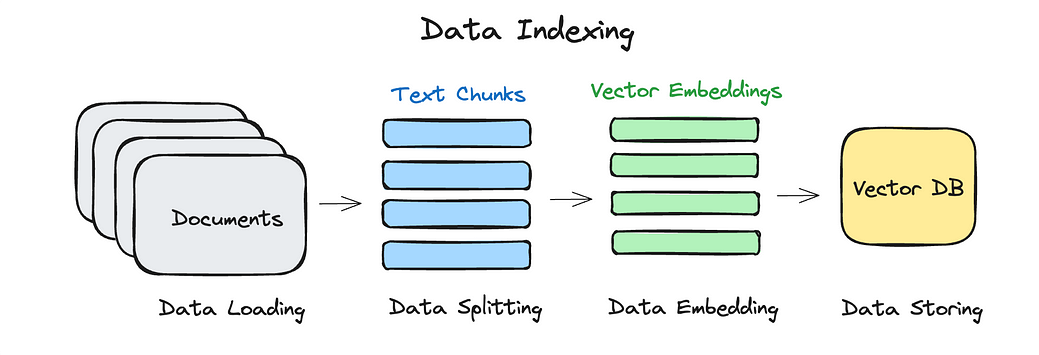
\includegraphics[width=0.8\textwidth]{images/Indexing_RAG.png}
  \caption{Indexing process} % Starred version
  \label{fig:indexing-process-manual}
\end{figure}


\section{Modeling} % Will auto-number as 5.4
\subsection{RAG Architecture Overview}
\label{subsec:rag-architecture}

Retrieval-Augmented Generation (RAG) is a hybrid architecture that combines dense document retrieval with generative language models to produce grounded and context-aware answers, as illustrated in Figure 3, which shows the complete pipeline from user query to final response.


\subsubsection*{Core Components}
\begin{itemize}
    \item \textbf{Retriever:} Retrieves relevant documents from a knowledge base using semantic similarity.
    \item \textbf{Generator:} Generates the final answer using the user's query and the retrieved context.
\end{itemize}

\subsubsection*{Workflow}
\begin{enumerate}
    \item \textbf{Query Encoding:}
    The user's question is first embedded into a dense vector using the \texttt{Bge-m3} embedding model, which captures the semantic meaning of the input.
    
    \item \textbf{Document Retrieval:}
    The query vector is used to search the \texttt{ChromaDB} vector store, where document chunks have also been embedded and indexed. The system retrieves the top-$k$ most relevant chunks based on cosine similarity.
    
    \item \textbf{Context Injection:}
    The retrieved chunks are concatenated and formatted as part of the prompt. This contextual information is added before the query to give the language model background knowledge it can reference during generation.
    
    \item \textbf{Response Generation:}
    The prompt, consisting of both the retrieved content and the original query, is passed to the LLM (\texttt{Llama3-2B-Instruct}), which generates a coherent and grounded response. The generated answer is influenced by the evidence provided, increasing factual accuracy.
\end{enumerate}

\subsubsection*{Advantages}
\begin{itemize}
    \item \textbf{Improved Factual Accuracy:} Since answers are based on up-to-date, verified documents, the model is less likely to hallucinate or fabricate information.
    
    \item \textbf{Dynamic Knowledge Updates:} New content can be added to the vector store without needing to retrain the model, allowing continuous updates and scalability.
    
    \item \textbf{Transparent Reasoning:} Retrieved chunks can be shown alongside responses, allowing users (including patients and doctors) to trace the origin of the information and validate it.
    
    \item \textbf{Domain Adaptability:} RAG can be easily tailored to specific domains like medical information, making it highly suitable for our use case involving respiratory health.
\end{itemize}

\begin{figure}[htbp]
  \centering
  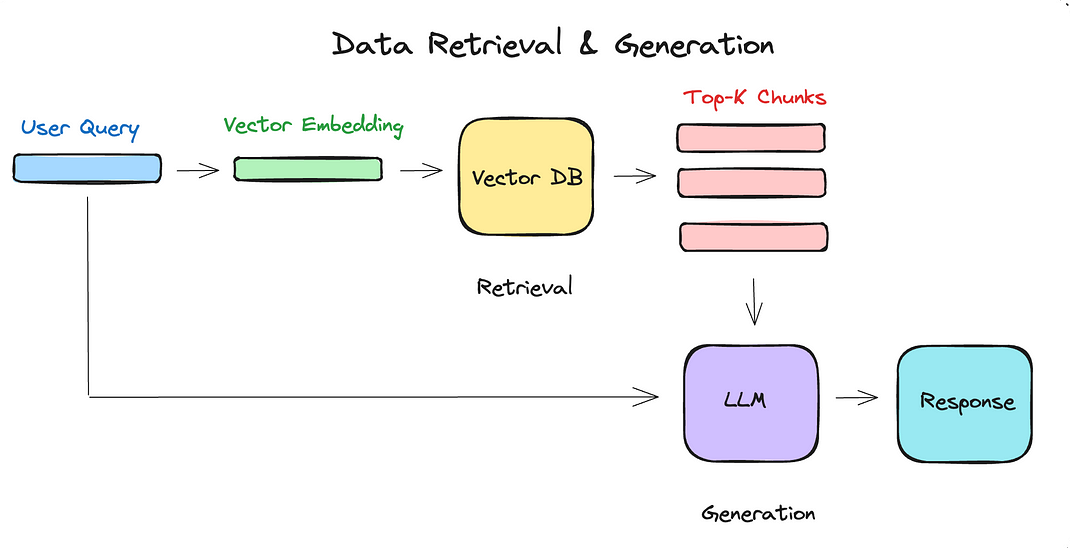
\includegraphics[width=0.8\textwidth]{images/Data_retrieval_and_generation_RAG.png}
  \caption*{\textbf{Figure 3:} RAG Pipeline} % Starred version
  \label{fig:indexing-process-manual}
\end{figure}

\subsection{Retriever Component}
\label{subsec:retriever}

The retriever is a critical part of the RAG pipeline responsible for identifying and returning the most semantically relevant document chunks in response to user queries.

We implemented a \textbf{dense retriever}, which relies on representing both queries and documents as dense vectors in a shared embedding space. Unlike traditional sparse retrieval methods (e.g., TF-IDF or BM25) that depend on exact keyword matching, dense retrieval captures semantic similarity by measuring the distance between vector representations. This allows retrieval of relevant information even when the exact query terms are not present in the documents.

\subsubsection*{Dense Retriever Mechanism}
Both the query $q$ and each document chunk $d_i$ are embedded into dense vectors:

\begin{equation*}
\mathbf{v}_q = \text{Embed}(q), \quad \mathbf{v}_{d_i} = \text{Embed}(d_i)
\end{equation*}

where $\text{Embed}(\cdot)$ is the embedding function implemented by the \texttt{BGE-M3} model.

The similarity score between the query and each document chunk is computed using cosine similarity:

\begin{equation*}
\text{sim}(\mathbf{v}_q, \mathbf{v}_{d_i}) = \frac{\mathbf{v}_q \cdot \mathbf{v}_{d_i}}{\|\mathbf{v}_q\| \|\mathbf{v}_{d_i}\|}
\end{equation*}

The retriever then ranks all candidate documents based on their similarity scores and selects the top-$k$ documents with the highest scores.

\subsubsection*{Embedding Model: BGE-M3}
To generate these embeddings, we used the \texttt{BGE-M3} embedding model developed by BAAI. This model was selected due to its strong capabilities:

\begin{itemize}
    \item \textbf{Multi-Functionality:} Supports dense retrieval, sparse retrieval, and multi-vector retrieval, making it versatile for different search scenarios.
    
    \item \textbf{Multi-Linguality:} Trained on over 100 languages, enabling support for diverse user inputs.
    
    \item \textbf{Multi-Granularity:} Handles inputs ranging from short queries to long documents (up to 8192 tokens), which suits embedding medical literature and user queries effectively.
\end{itemize}

These characteristics allow \texttt{BGE-M3} to generate rich, meaningful embeddings that improve retrieval quality.

\subsubsection*{Top-K Selection}
The retriever selects the top 3 most relevant document chunks for each query based on cosine similarity between embeddings. This choice was made after analyzing the collected queries and frequently asked questions (FAQ). We found that no more than three documents were generally necessary to provide sufficient context for answering user queries accurately. Setting top-k = 3 balances providing enough relevant information while avoiding excessive or noisy context that could confuse the language model.
This approach ensures the generator receives focused and contextually relevant information, improving the overall response quality.

\subsection{Generator Component}
\label{subsec:generator}

\subsubsection{Language Model Description}
\label{sssec:lm-description}

We used in the generator component the Llama 3.2 1B Instruct model with Q6-K quantization. This model contains approximately 1 billion parameters, offering a balance between computational efficiency and language understanding capabilities. It is specifically fine-tuned on instruction-following datasets, which enables it to interpret and respond effectively to user queries with clear, context-aware, and relevant answers.
The model benefits from Q6-K quantization, a technique that reduces the precision of model weights to 6 bits, allowing for significant reductions in memory usage and faster inference times without substantially sacrificing performance. This makes the model well-suited for deployment in resource-constrained environments, such as mobile applications.
The Llama 3.2 1b Instruct model’s combination of compact size, instruction fine-tuning, and efficient quantization makes it ideal for our AI assistant, enabling fast and reliable generation of medically accurate responses in real-time.


\subsubsection{Instruct-Tuning}
\label{sssec:instruct-tuning}

\paragraph{Objective:} 
 The fine-tuning process aimed to adapt the Llama 3.2 model for instruction-following tasks, enhancing its ability to generate accurate and context-aware responses based on user queries.

\paragraph{Fine-Tuning Methodology:}
Meta employed a combination of Supervised Fine-Tuning (SFT) and Reinforcement Learning with Human Feedback (RLHF) to align the model's outputs with human preferences for helpfulness and safety.

\begin{itemize}
    \item \textbf{Supervised Fine-Tuning (SFT):}
    In this phase, the model was trained on a dataset comprising instruction-response pairs. This supervised approach helped the model learn to follow instructions and generate appropriate responses.
    
    \item \textbf{Reinforcement Learning with Human Feedback (RLHF):}
    Following SFT, RLHF was utilized to further refine the model's behavior. Human feedback was incorporated to guide the model towards producing outputs that align with desired characteristics, such as factual accuracy and helpfulness.
\end{itemize}

\paragraph{Training Data:}
The fine-tuning process utilized a diverse mix of publicly available online data, encompassing various languages and domains. This multilingual dataset enabled the model to perform effectively across different languages and tasks .

\paragraph{Outcome:}
The fine-tuned Llama 3.2 Instruct models demonstrated improved performance on common industry benchmarks, outperforming many existing open-source and closed chat models in tasks requiring instruction-following capabilities .

\subsubsection{Quantization}
\label{sssec: quantization}

Quantization is a widely used technique in deep learning to reduce the computational and memory costs of neural networks by representing weights and activations with lower precision numerical formats. Instead of using 32-bit floating-point numbers (FP32), quantization typically converts these values to 16-bit (FP16), 8-bit, or even lower-bit integer representations such as 6-bit or 4-bit integers.
In our project, we employed \texttt{Q6\_K} quantization, which specifically compresses model weights to 6-bit precision, allowing a significant reduction in model size and inference latency while maintaining strong performance.

\paragraph{Techniques in Quantization:}
There are several methods for quantization, including:

\begin{itemize}
    \item \textbf{Post-Training Quantization (PTQ):} This technique applies quantization after the model has been fully trained. It is fast and does not require retraining but can sometimes lead to accuracy degradation if not carefully tuned.
    
    \item \textbf{Quantization-Aware Training (QAT):} In this method, the model is trained or fine-tuned with quantization in mind. The training simulates quantized weights and activations, helping the model adapt to the lower precision and thus preserving accuracy better.
\end{itemize}

Our use of \texttt{Q6\_K} falls into post-training quantization optimized for language models, focusing on balancing compression and accuracy without retraining the entire model.

\paragraph{How Quantization Works:}
The core idea is to map floating-point weights $w \in \mathbb{R}$ to discrete quantized values $q \in \mathbb{Z}$ using a scale $s$ and zero-point $z$, typically by:

\begin{equation*}
q = \text{round}\left(\frac{w}{s}\right) + z
\end{equation*}

where $s$ scales the real values into the quantization range and $z$ shifts the zero point. In 6-bit quantization, the values are mapped to integers in the range $[0, 63]$.

For inference, the quantized weights are dequantized back to floating-point by:

\begin{equation*}
\hat{w} = s \times (q - z)
\end{equation*}

The challenge is to choose $s$ and $z$ such that the quantized weights closely approximate the original weights and minimize error propagation through the network.

\paragraph{Benefits of Q6\_K Quantization:}
\begin{itemize}
    \item \textbf{Memory Reduction:} Reducing the weight precision from 32-bit to 6-bit reduces model size by over 5 times.
    
    \item \textbf{Inference Speedup:} Integer arithmetic operations on 6-bit numbers are faster and more energy-efficient on compatible hardware.
    
    \item \textbf{Compatibility:} \texttt{Q6\_K} quantization is designed specifically for transformer architectures, preserving their performance better than naïve quantization approaches.
    
    \item \textbf{Minimal Accuracy Loss:} Carefully calibrated quantization parameters help maintain the semantic understanding and generation quality of the language model.
\end{itemize}

\paragraph{Challenges}
\begin{itemize}
    \item \textbf{Quantization Error:} Low-bit precision introduces quantization noise which can degrade model output if not carefully managed.
    
    \item \textbf{Hardware Support:} Efficient execution of 6-bit operations requires specialized hardware or optimized libraries, which might not be universally available.
    
    \item \textbf{Calibration:} Choosing appropriate scale and zero-point parameters requires calibration on representative data to minimize performance loss.
\end{itemize}

Overall, \texttt{Q6\_K} quantization provides an effective trade-off between resource efficiency and model performance, making it highly suitable for deploying \texttt{Llama 3.2 1B Instruct} in our AI assistant, ensuring fast, reliable, and resource-conscious inference.

\subsubsection{Prompt Engineering}
\label{sssec:prompt-engineering}

Prompt engineering is the process of designing and structuring the input provided to a language model to effectively guide its behavior and output. It plays a critical role in ensuring the model understands the task objective, responds appropriately, and uses the provided context efficiently.

In our RAG-based assistant, prompt engineering was essential to help the language model generate relevant, fact-based, and context-aware answers.

\paragraph{System Prompt Design}
We defined a system prompt to instruct the model on its role and expected tone. This was used to prime the model at the beginning of each interaction.

\begin{verbatim}
You are a knowledgeable and compassionate medical assistant chatbot 
specialized in respiratory diseases. Your goal is to help users understand 
symptoms, conditions, prevention, and treatments related to the respiratory 
system. Always provide clear, concise, and medically accurate information 
based on trusted sources. Avoid repetition, stay focused on the specific 
question, and include practical advice when relevant.
\end{verbatim}

This guided the model to behave as a reliable assistant, aligned with the medical nature of the application.

\paragraph{Contextual Prompt Construction} 
When a user submits a query, the top-3 most relevant chunks from the knowledge base are retrieved and injected into the prompt following this structure:

\begin{verbatim}
Question: [User's original question]
Context:
1. [First retrieved knowledge chunk]
2. [Second retrieved knowledge chunk] 
3. [Third retrieved knowledge chunk]

Instruction: Use only the provided context to answer. 
If information is incomplete, respond: "Based on my medical resources, 
I would suggest consulting a healthcare professional about this."
Never speculate beyond the given context.
\end{verbatim}

The prompt explicitly instructs the LLM to: (1) treat the context as primary source but verify completeness, (2) acknowledge limitations when context is insufficient by recommending professional consultation, and (3) strictly avoid fabrication. This design ensures trustworthy responses while minimizing hallucinations and maintaining clinical responsibility - particularly crucial for respiratory health queries where accuracy impacts patient outcomes.

This design ensures that responses are fact-grounded, transparent, and aligned with medical best practices.
\section{Evaluation} % Will auto-number as 5.5
\subsection{Retriever Evaluation}
\label{subsec:retriever-eval}

The retriever component plays a crucial role in the Retrieval-Augmented Generation (RAG) pipeline. It is responsible for selecting the most relevant pieces of information (chunks) from a large corpus in response to a user query. To evaluate its effectiveness, we used several well-established metrics from the information retrieval field.

\subsubsection{Evaluation Metrics}
\begin{itemize}
    \item \textbf{Mean Reciprocal Rank (MRR):}
    The MRR evaluates how highly the first relevant document appears in the ranked list of retrieved documents. For each query, the reciprocal rank is calculated as:
    
    \begin{equation*}
    \text{Reciprocal Rank} = \frac{1}{\text{rank of the first relevant document}}
    \end{equation*}
    
    Then, the MRR is the average of these reciprocal ranks across all queries:
    
    \begin{equation*}
    \text{MRR} = \frac{1}{|Q|} \sum_{i=1}^{|Q|} \frac{1}{\text{rank}_i}
    \end{equation*}
    
    A higher MRR (closer to 1) indicates that the system often retrieves the correct document in the top position, which is critical for user-facing applications.

    \item \textbf{Mean Average Precision (MAP):}
    MAP considers all relevant documents, not just the first one. For each query, it calculates the average precision across the retrieved results and then averages over all queries. It is defined as:
    
    \begin{equation*}
    \text{MAP} = \frac{1}{|Q|} \sum_{i=1}^{|Q|} \left( \frac{1}{m_i} \sum_{k=1}^{n} P(k) \cdot rel(k) \right)
    \end{equation*}
    
    Where:
    \begin{itemize}
        \item $P(k)$ is the precision at cut-off $k$
        \item $rel(k)$ is a binary indicator of relevance at position $k$
        \item $m_i$ is the total number of relevant documents for query $i$
    \end{itemize}
    
    This metric rewards systems that rank all relevant documents highly.

    \item \textbf{Recall@K (e.g., Recall@3):}
    Recall@K measures how many relevant documents are retrieved among the top K results. It is computed as:
    
    \begin{equation*}
    \text{Recall@K} = \frac{\text{\# of relevant documents in top K}}{\text{Total \# of relevant documents}}
    \end{equation*}
    \\
    In this project, we used Recall@3 since the retriever was configured to return Top-K = 3 documents. This value was chosen based on manual analysis of a dataset of FAQs and real user queries, where it was observed that most answers could be accurately supported using at most three context documents.
\end{itemize}

\subsubsection{Global MRR Benchmark Evaluation}
The dense retriever leveraging the \texttt{BGE-M3} embedding model was evaluated on a multilingual MRR benchmark dataset. The results demonstrate that \texttt{BGE-M3} consistently outperformed other embedding models across multiple languages, showcasing its strong generalization and retrieval capabilities.

The MRR scores achieved by \texttt{BGE-M3} on different languages are as follows:
\begin{itemize}
    \item English: 0.68
    \item French: 0.60
    \item Hungarian (HU): 0.64
    \item Czech (CS): 0.65
\end{itemize}

These scores highlight the model's robust ability to retrieve relevant documents effectively in various linguistic contexts, which is crucial for building a reliable AI assistant. The comparative performance is illustrated in Figure~\ref{fig:mrr-benchmark}, which clearly shows \texttt{BGE-M3} leading other tested models on this benchmark.
\begin{figure}[htbp]
  \centering
  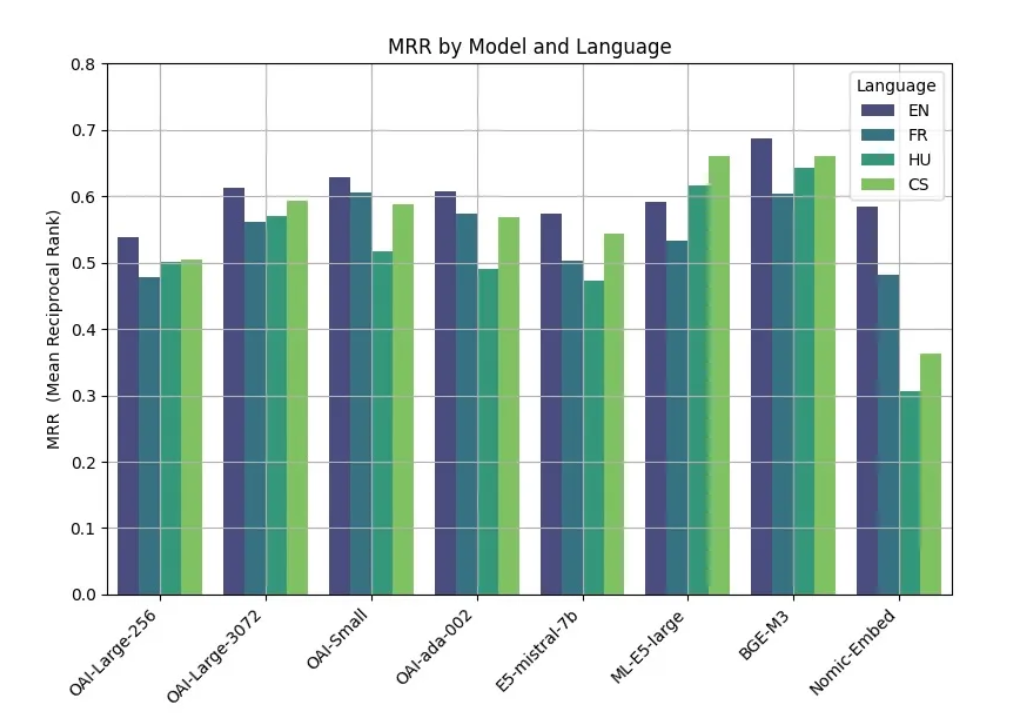
\includegraphics[width=0.8\textwidth]{images/MRR.png}
  \caption{MRR Benchmark results} % Starred version
  \label{fig:mrr-benchmark}
\end{figure}


\subsubsection{Domain Evaluation}
For evaluating the retriever’s performance in the context of respiratory diseases, we created a dedicated evaluation dataset. This dataset includes approximately 50 manually selected questions related to common respiratory conditions, symptoms, and treatments. The questions were gathered from verified sources such as medical forums, FAQs, and healthcare websites to reflect real-world user inquiries. \\
We conducted a detailed manual analysis to determine which documents are relevant for answering each question. This involved reviewing the retrieved documents and annotating those essential for fully understanding the queries. This process also helped us identify the optimal number of relevant documents per question, informing retrieval parameter choices such as the top-k value. \\
This manual curation provides a high-quality ground truth for evaluation, allowing precise assessment of retriever performance in our specific domain.

The retriever achieved \textbf{exceptional performance} on our respiratory disease dataset:
\vspace{0.5em}
\hrule
\begin{itemize}
    \item \textbf{Mean Reciprocal Rank (MRR):} \textbf{0.72} 
    \item \textbf{Mean Average Precision (MAP):} \textbf{0.68}
    \item \textbf{Recall@3:} \textbf{0.75}
\end{itemize}
\hrule
\vspace{0.5em}

These scores demonstrate the retriever’s effectiveness in ranking relevant documents higher, which is critical for accurate and context-aware AI assistant responses. The strong performance reflects the suitability of our embedding model and retrieval strategy tuned to the domain.\\
Nonetheless, some questions involving rare or highly specialized information showed slightly lower precision, highlighting areas for potential improvement. Overall, the results confirm that our retriever performs well in the respiratory disease domain and supports the AI assistant’s effectiveness.

\subsection{End-to-End System Evaluation}
\label{subsec:e2e-eval}

To assess the end-to-end effectiveness of our Retrieval-Augmented Generation (RAG) system, we applied the \textit{LLM-as-a-Judge} technique, where a powerful large language model evaluates generated answers using a structured rubric. Specifically, we employed \texttt{GPT-4} as an automatic evaluator to review responses generated by our system for a carefully curated set of 50 domain-specific questions.\\
As depicted in Figure~\ref{fig:llm-judge}, the evaluation pipeline feeds the user question, the RAG-generated response, and—where applicable—the baseline response into the judge model. GPT-4.0 then rates the answers on six essential dimensions, each on a scale from 0 to 10:
\begin{itemize}
    \item \textbf{Groundedness:} Alignment with retrieved context
    \item \textbf{Correctness:} Factual and domain accuracy
    \item \textbf{Coherence:} Clarity, structure, and logical flow
    \item \textbf{Relevance:} Direct response to query
    \item \textbf{Novelty:} Added value from synthesis
    \item \textbf{Overall Score:} General utility and effectiveness
\end{itemize}
\begin{figure}[htbp]
  \centering
  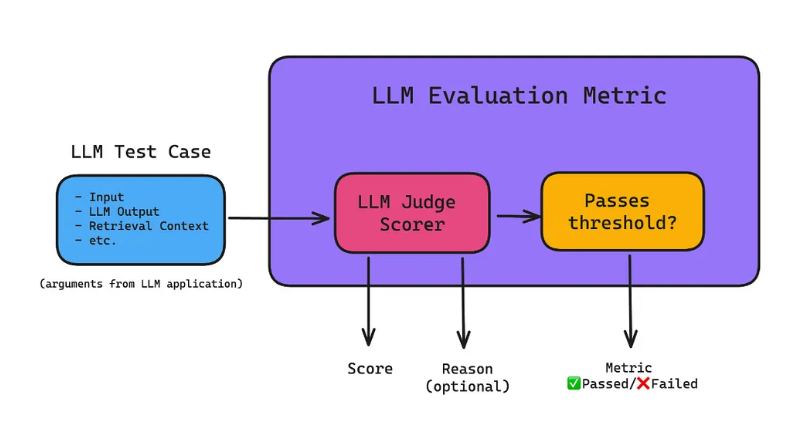
\includegraphics[width=0.8\textwidth]{images/LLM_AS_JUDGE.png}
  \caption{LLM Evaluation process} % Starred version
  \label{fig:llm-judge}
\end{figure}
\\
\begin{table}[h]
    \centering
    \begin{tabular}{lcc}
        \toprule
        \textbf{Metric} & \textbf{RAG System} & \textbf{Baseline} \\
        \midrule
        Groundedness & 8.7 & 5.2 \\
        Correctness & 8.5 & 5.8 \\
        Coherence & 9.1 & 8.7 \\
        Relevance & 8.9 & 6.3 \\
        Novelty & 7.8 & 6.9 \\
        Overall Score & 8.6 & 6.4 \\
        \bottomrule
    \end{tabular}
    \caption{Performance comparison: RAG vs. Baseline (50 questions)}
    \label{tab:rag-vs-baseline}
\end{table}

To quantify the contribution of retrieval, we compared our RAG system with a baseline model that used the same Llama 3.2 1B Instruct LLM but without any contextual documents. The average scores across the 50-question evaluation set are shown in Table~\ref{tab:rag-vs-baseline}.

As observed in Table 1, the RAG system consistently outperformed the baseline across all metrics. The most substantial gains were seen in groundedness, correctness, and relevance, confirming that access to relevant, retrieved context significantly enhances the LLM’s ability to generate reliable and precise answers. While coherence remained relatively high in both cases, the RAG version improved the interpretability and factual grounding of responses, making it better suited for medical assistance applications.
\section{Deployment} % Will auto-number as 5.6
To make the system accessible and efficient in a real-world setting, we designed a lightweight and modular deployment architecture. The deployment stack ensures that both the LLM and embedding-based retrieval components are available through a simple API interface.

\textbf{Ollama for Model Serving:}
We used Ollama to serve both the Llama 3.2 1B Instruct model and the BGE-M3 embedding model locally. Ollama provides an efficient and GPU-friendly environment to run quantized models with minimal overhead, which helped achieve low-latency responses during generation and retrieval.

\textbf{FastAPI for Backend Interface:}
A FastAPI server was built to act as a communication layer between the front end and the core RAG system. This backend handles user queries, performs retrieval using the embedding model, generates responses via the LLM, and returns structured answers to the front end.

\textbf{Docker for Containerization:}
To ensure portability and ease of deployment, the entire backend system (including FastAPI and Ollama runtime) was packaged into a Docker container. This allows consistent deployment across environments and simplifies maintenance and scaling.

This deployment setup strikes a balance between efficiency and simplicity, making the AI assistant suitable for both development and production testing scenarios.

\section*{Conclusion}
This chapter outlined the development of our AI assistant powered by a Retrieval-Augmented Generation (RAG) system. From concept to deployment, the focus was on creating a helpful, reliable, and multilingual tool to assist users with respiratory health questions. The results demonstrate the potential of combining retrieval with generation to provide informative and grounded answers, while always emphasizing the importance of professional medical advice.




\setcounter{chapter}{5} 
\chapter{Implementation} % This will automatically be Chapter 5
\label{chap:implementation}


\section*{Introduction}
\addcontentsline{toc}{section}{Introduction}

This chapter presents the implementation phase of our project: an AI-powered mobile application designed to analyze breathing sounds and assist in detecting respiratory diseases.

The implementation phase translates theoretical concepts into a working system. It focuses on the tools, technologies, and methodologies used to build the application and ensure its reliability and performance.

The core objective is to develop a mobile app capable of recording respiratory audio, uploading it securely, and using AI-based models to provide preliminary diagnostic feedback. The app also allows users to upload medical reports and offers a simple, intuitive interface with real-time insights.

To achieve this, we adopted a modular architecture that separates mobile development, backend services, and AI inference. The mobile app was developed using Flutter, chosen for its cross-platform capabilities and development speed. Appwrite was selected as the backend platform for its support of authentication, storage, and serverless functions.

This chapter begins with an overview of the system architecture and its components. It then details the implementation of key modules, including audio capture and encryption, data transmission, backend integration, and AI model deployment. Each section highlights the technical decisions made and the reasoning behind them.

\pagebreak  % Forces a new page
\section{System Architecture}
\label{sec:system_architecture}

The system architecture of our AI-powered mobile application is designed to ensure modularity, scalability, and secure data handling. It is composed of three main components: the mobile application, the backend services, and the AI inference engine. Each component plays a distinct role while communicating seamlessly with the others.

The architecture follows a modular pattern to facilitate independent development and testing of each module. This design choice improves maintainability and simplifies the integration of additional features in the future.

The overall system structure is illustrated in Figure~\ref{fig:system-architecture}, which outlines the interactions between the core components of the application.


\begin{figure}[H]
    \centering
    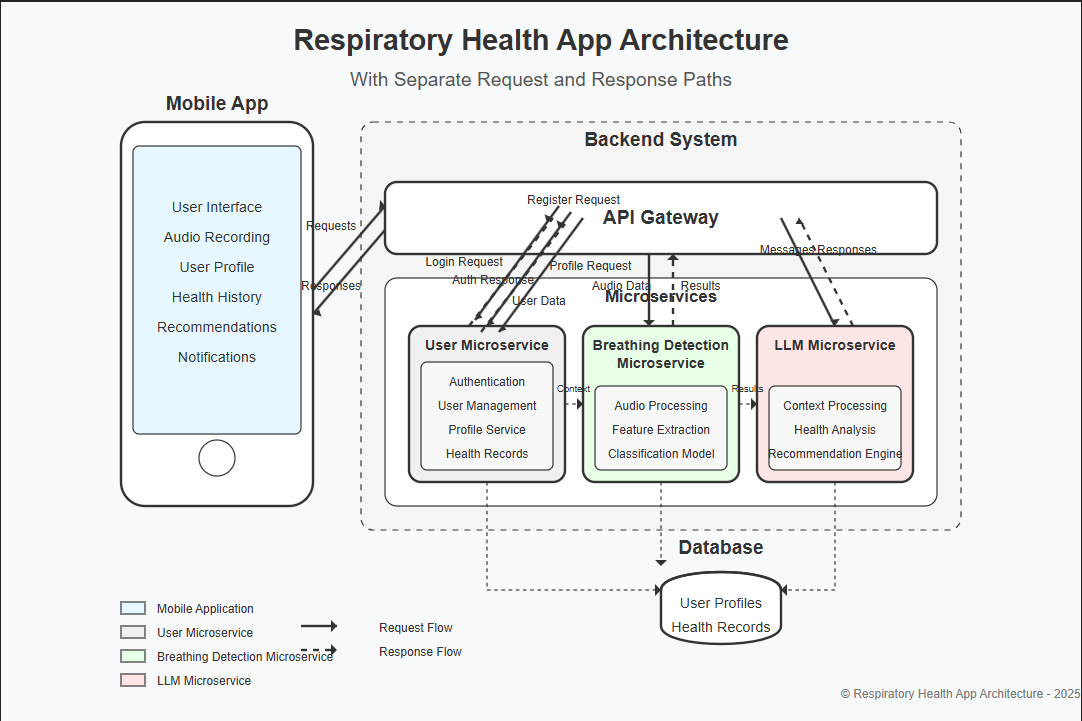
\includegraphics[width=\textwidth]{images/architecture.png}
    \caption{System Architecture of the AI-Powered Mobile Application}
    \label{fig:system-architecture}
\end{figure}

\subsubsection*{Mobile Application}

The mobile application, developed using Flutter, provides the user interface and handles client-side functionalities. These include audio recording, local encryption, file selection, and UI interactions. It also manages authentication and communication with the backend.

\subsubsection*{Backend Services}

The backend is powered by Appwrite, a self-hosted backend-as-a-service platform. It handles authentication, file storage (medical reports and audio), and serverless functions. Appwrite ensures secure and scalable data management while offering APIs that are easy to integrate with Flutter.

\subsubsection*{AI Inference Engine}

The AI inference module is responsible for analyzing respiratory audio data and generating preliminary diagnostic feedback. Once an audio file is uploaded and validated, it is sent to a dedicated inference server or function that runs a pre-trained deep learning model to detect anomalies in the breathing pattern.

\vspace{1em}

This modular architecture enables efficient development, enhances security, and supports the core functionality of respiratory disease detection.

\section{Mobile Application}
\label{sec:mobile_application}

The mobile application serves as the central user interface of our AI-powered respiratory analysis system. Built with Flutter, it offers a seamless and cross-platform experience. This section presents a walkthrough of the app’s core features, showcasing its design, functionality, and user flow.

\subsection{Visual Identity and Design Language}

The application embraces a medically inspired color palette referencing the official World Health Organization (WHO) guidelines, aiming for clarity, trust, and accessibility. The logo symbolizes the lungs through a stylized graphic, while the central dot represents a sensor tasked with detecting respiratory anomalies.

The primary branding elements, including both filled and outline logo variants, are shown in Figure~\ref{fig:app_logos}.

\begin{figure}[H]
    \centering
    
\includegraphics[width=0.25\textwidth]{images/UI_Screenshots/logo_filled.png}
    \hspace{2em}
    
\includegraphics[width=0.25\textwidth]{images/UI_Screenshots/logo_unfilled.png}
    \caption{Application Logos: Filled and Outline}
    \label{fig:app_logos}
\end{figure}

\subsection{Authentication: Login and Signup}

The user journey begins with secure authentication. A simple interface for logging in or signing up is provided, as seen in Figure~\ref{fig:login_screen}.

\begin{figure}[H]
    \centering
    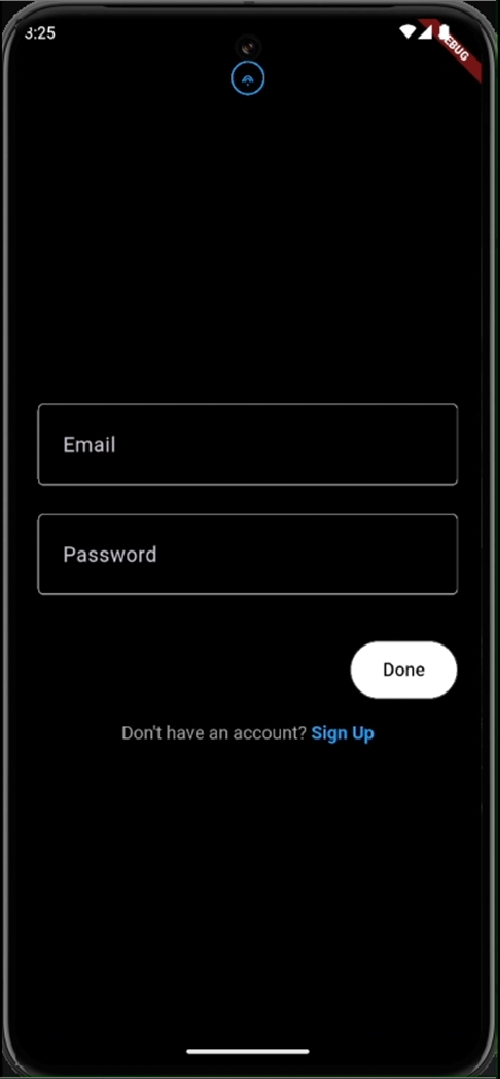
\includegraphics[width=0.35\textwidth]{images/UI_Screenshots/login_screen.png}
    \caption{Login Screen}
    \label{fig:login_screen}
\end{figure}

\subsection{User Profile Management}

Once authenticated, users are directed to a profile screen where they can view and manage their personal information. This interface is illustrated in Figure~\ref{fig:profile_screen}.

\begin{figure}[H]
    \centering
    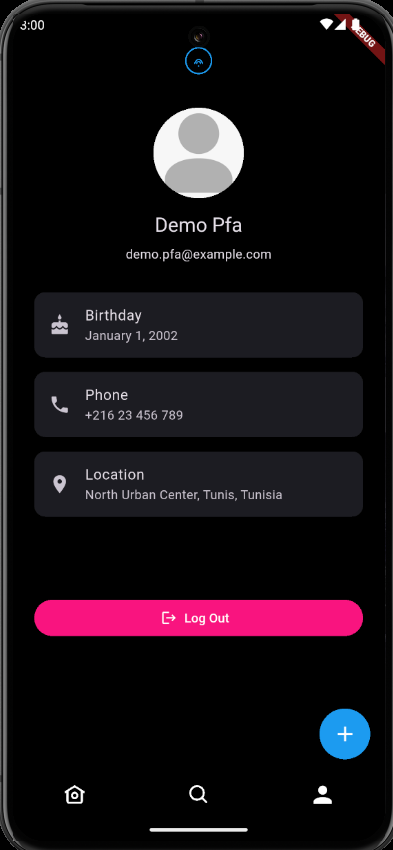
\includegraphics[width=0.35\textwidth]{images/UI_Screenshots/profile_screen.png}
    \caption{Profile Screen}
    \label{fig:profile_screen}
\end{figure}

\subsection{Home Screen – No Diagnoses Yet}

The initial home screen is presented when the user has not yet submitted any diagnoses. This clean interface is displayed in Figure~\ref{fig:home_screen_empty}.

\begin{figure}[H]
    \centering
    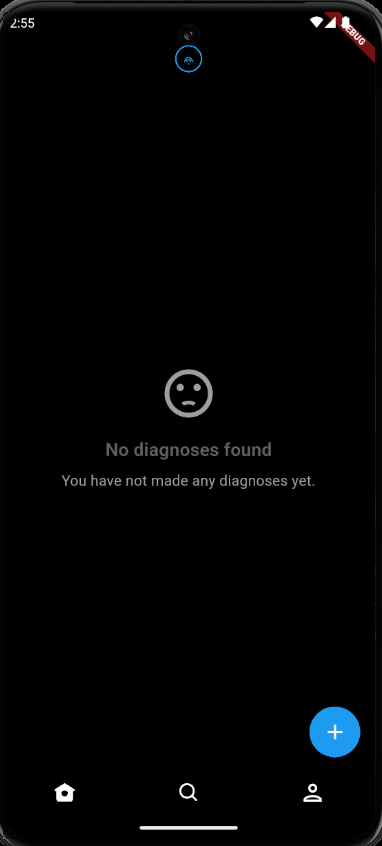
\includegraphics[width=0.35\textwidth]{images/UI_Screenshots/home_screen_no_diagnoses.png}
    \caption{Home Screen Without Diagnoses}
    \label{fig:home_screen_empty}
\end{figure}

\subsection{Search Screen – No History}

A search feature is available for reviewing past diagnoses. In the absence of history, the interface appears as shown in Figure~\ref{fig:search_screen_empty}.

\begin{figure}[H]
    \centering
    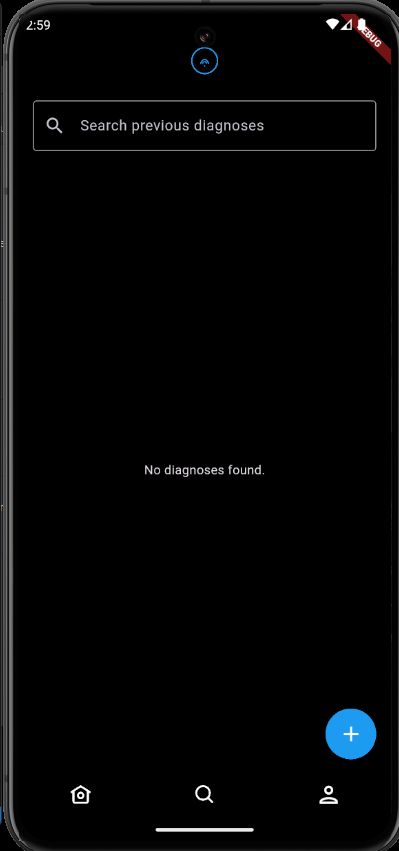
\includegraphics[width=0.35\textwidth]{images/UI_Screenshots/search_screen.png}
    \caption{Search Screen Without History}
    \label{fig:search_screen_empty}
\end{figure}

\subsection{Creating a New Diagnosis}

To start a diagnosis, users can record audio, upload medical files, and input symptoms using the interface shown in Figure~\ref{fig:create_diagnosis}.

\begin{figure}[H]
    \centering
    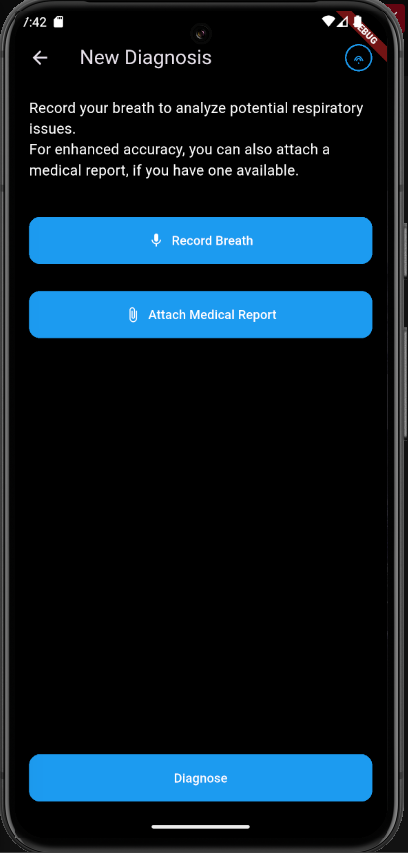
\includegraphics[width=0.35\textwidth]{images/UI_Screenshots/create_diagnosis_screen.png}
    \caption{Diagnosis Creation Interface}
    \label{fig:create_diagnosis}
\end{figure}

\subsection{Home Screen – With Previous Diagnoses}

After a diagnosis is performed, the home screen updates to reflect the user's diagnostic history, as demonstrated in Figure~\ref{fig:home_screen_with_history}.

\begin{figure}[H]
    \centering
    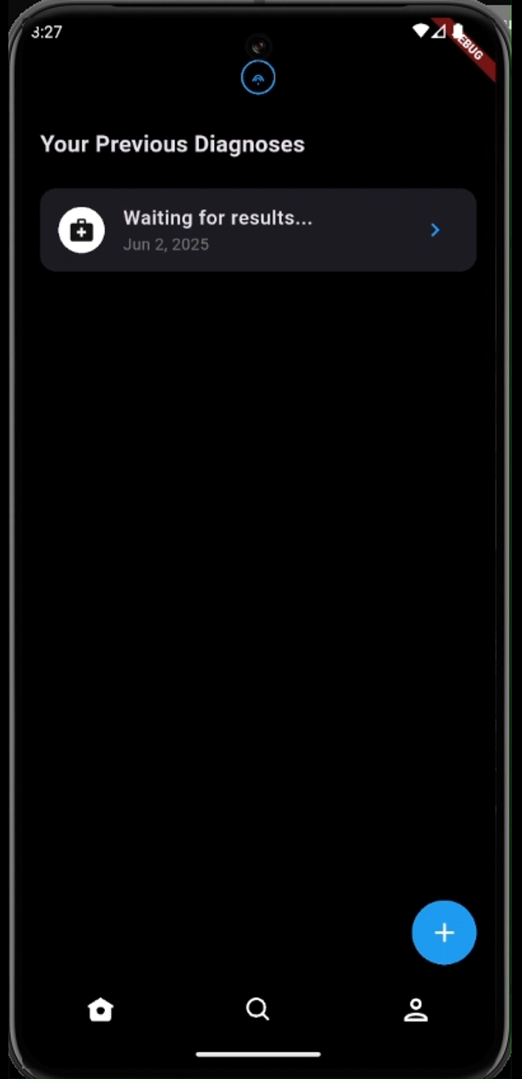
\includegraphics[width=0.35\textwidth]{images/UI_Screenshots/home_screen_with_previous_diagnoses.png}
    \caption{Home Screen Displaying Previous Diagnoses}
    \label{fig:home_screen_with_history}
\end{figure}

\subsection{Diagnosis Details – Waiting for Results}

Once a new diagnosis is submitted, the system informs the user that the analysis is in progress. This intermediate state is depicted in Figure~\ref{fig:diagnosis_waiting}.

\begin{figure}[H]
    \centering
    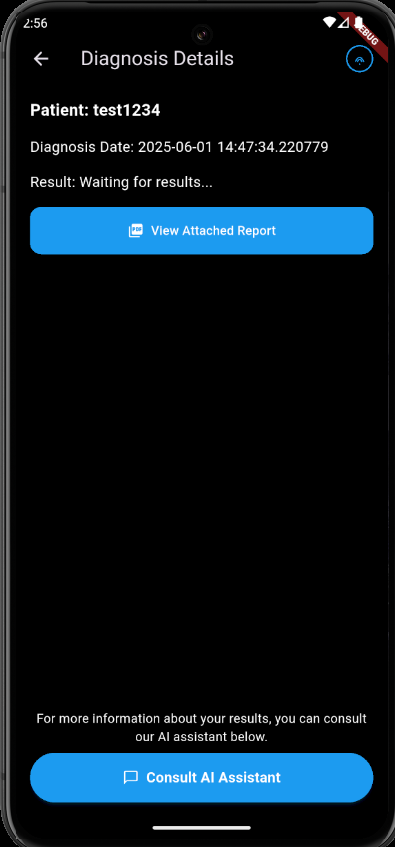
\includegraphics[width=0.35\textwidth]{images/UI_Screenshots/diagnosis_details_screen_waiting_for_results.png}
    \caption{Diagnosis Details – Awaiting AI Analysis}
    \label{fig:diagnosis_waiting}
\end{figure}

\subsection{Diagnosis Details – Results Ready}

After analysis is complete, users are presented with detailed diagnostic feedback, as shown in Figure~\ref{fig:diagnosis_results}.

\begin{figure}[H]
    \centering
    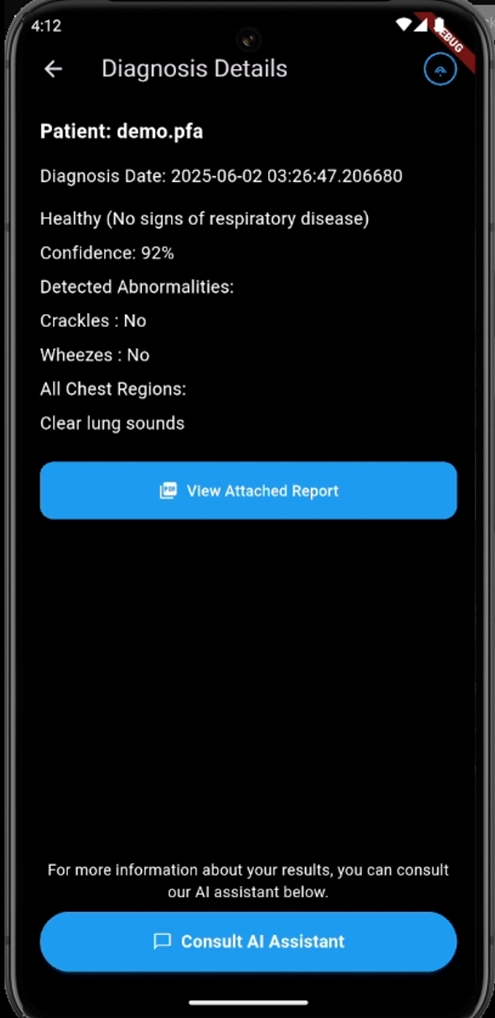
\includegraphics[width=0.35\textwidth]{images/UI_Screenshots/diagnosis_details_screen_results_ready.png}
    \caption{Diagnosis Details – Results Ready}
    \label{fig:diagnosis_results}
\end{figure}

\subsection{AI Assistant Onboarding}

When consulting the AI assistant for the first time, users are guided through an onboarding screen that outlines its purpose, as illustrated in Figure~\ref{fig:ai_onboarding}.

\begin{figure}[H]
    \centering
    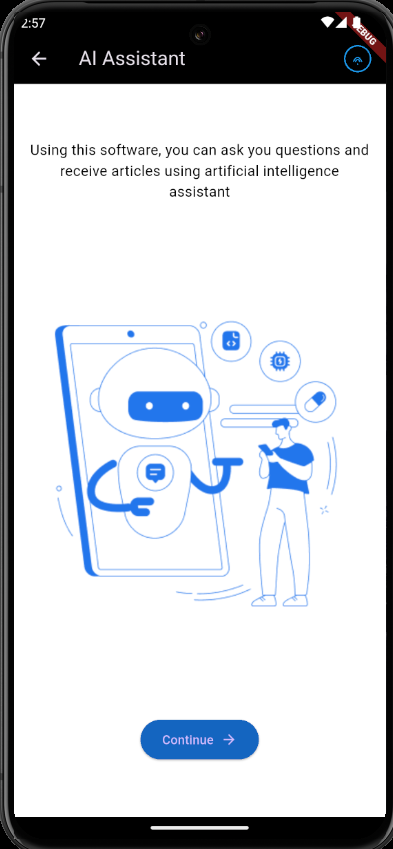
\includegraphics[width=0.35\textwidth]{images/UI_Screenshots/on_boarding_ai_assistant_screen.png}
    \caption{AI Assistant Onboarding Screen}
    \label{fig:ai_onboarding}
\end{figure}

\subsection{AI Assistant – Start Screen}

Following onboarding, users arrive at a starting interface that invites medical queries, as depicted in Figure~\ref{fig:ai_start}.

\begin{figure}[H]
    \centering
    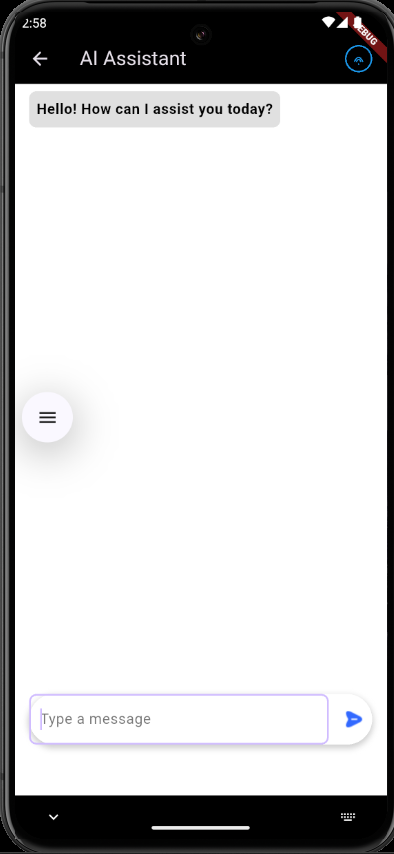
\includegraphics[width=0.35\textwidth]{images/UI_Screenshots/ai_assistant_screen_starting_screen.png}
    \caption{AI Assistant – Starting Interface}
    \label{fig:ai_start}
\end{figure}

\subsection{AI Assistant – Chat Interface}

The assistant responds in a conversational style, as shown in Figure~\ref{fig:ai_chat}, providing interactive, medically grounded guidance.

\begin{figure}[H]
    \centering
    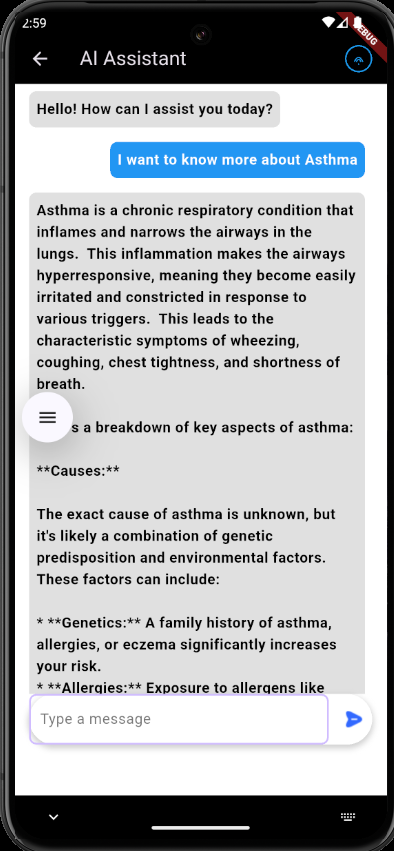
\includegraphics[width=0.35\textwidth]{images/UI_Screenshots/ai_assistant_screen_chat_example.png}
    \caption{AI Assistant Chat Interaction}
    \label{fig:ai_chat}
\end{figure}

\subsection{Summary}

The mobile application was designed to deliver a smooth, medically reliable, and user-centric experience. Each screen plays a specific role in guiding the user through authentication, diagnosis creation, result review, and AI consultation. Leveraging Flutter, the app ensures cross-platform consistency and accessibility. The clear design, inspired by WHO standards, and the integration of visual cues like the lung-symbol logo reinforce its identity as a trusted respiratory health tool.

\newpage

\section{Backend and API Integration}
\label{sec:backend_api}

The backend infrastructure is a critical component of our AI-powered mobile application, enabling secure data handling, user management, and seamless communication between the mobile client and AI services. Built around Appwrite—a self-hosted backend-as-a-service (BaaS) platform—the system benefits from a robust, modular, and scalable architecture.

\subsection{Appwrite as Backend-as-a-Service (BaaS)}

Appwrite serves as the core backend platform, providing essential services such as authentication, database storage, file handling, serverless computing, and real-time updates. It supports structured data for user profiles and health records, encrypted storage for audio and medical files, and custom functions for executing AI-based health analysis.

The architecture shown in Figure~\ref{fig:appwrite_backend} depicts how the Flutter-based mobile frontend communicates with Appwrite services over secure HTTPS, enabling a seamless flow of authentication, data storage, and diagnostic processing. Each backend service operates independently while being orchestrated via the Appwrite API Gateway, which manages routing and authentication for all client requests.

\begin{figure}[H]
    \centering
    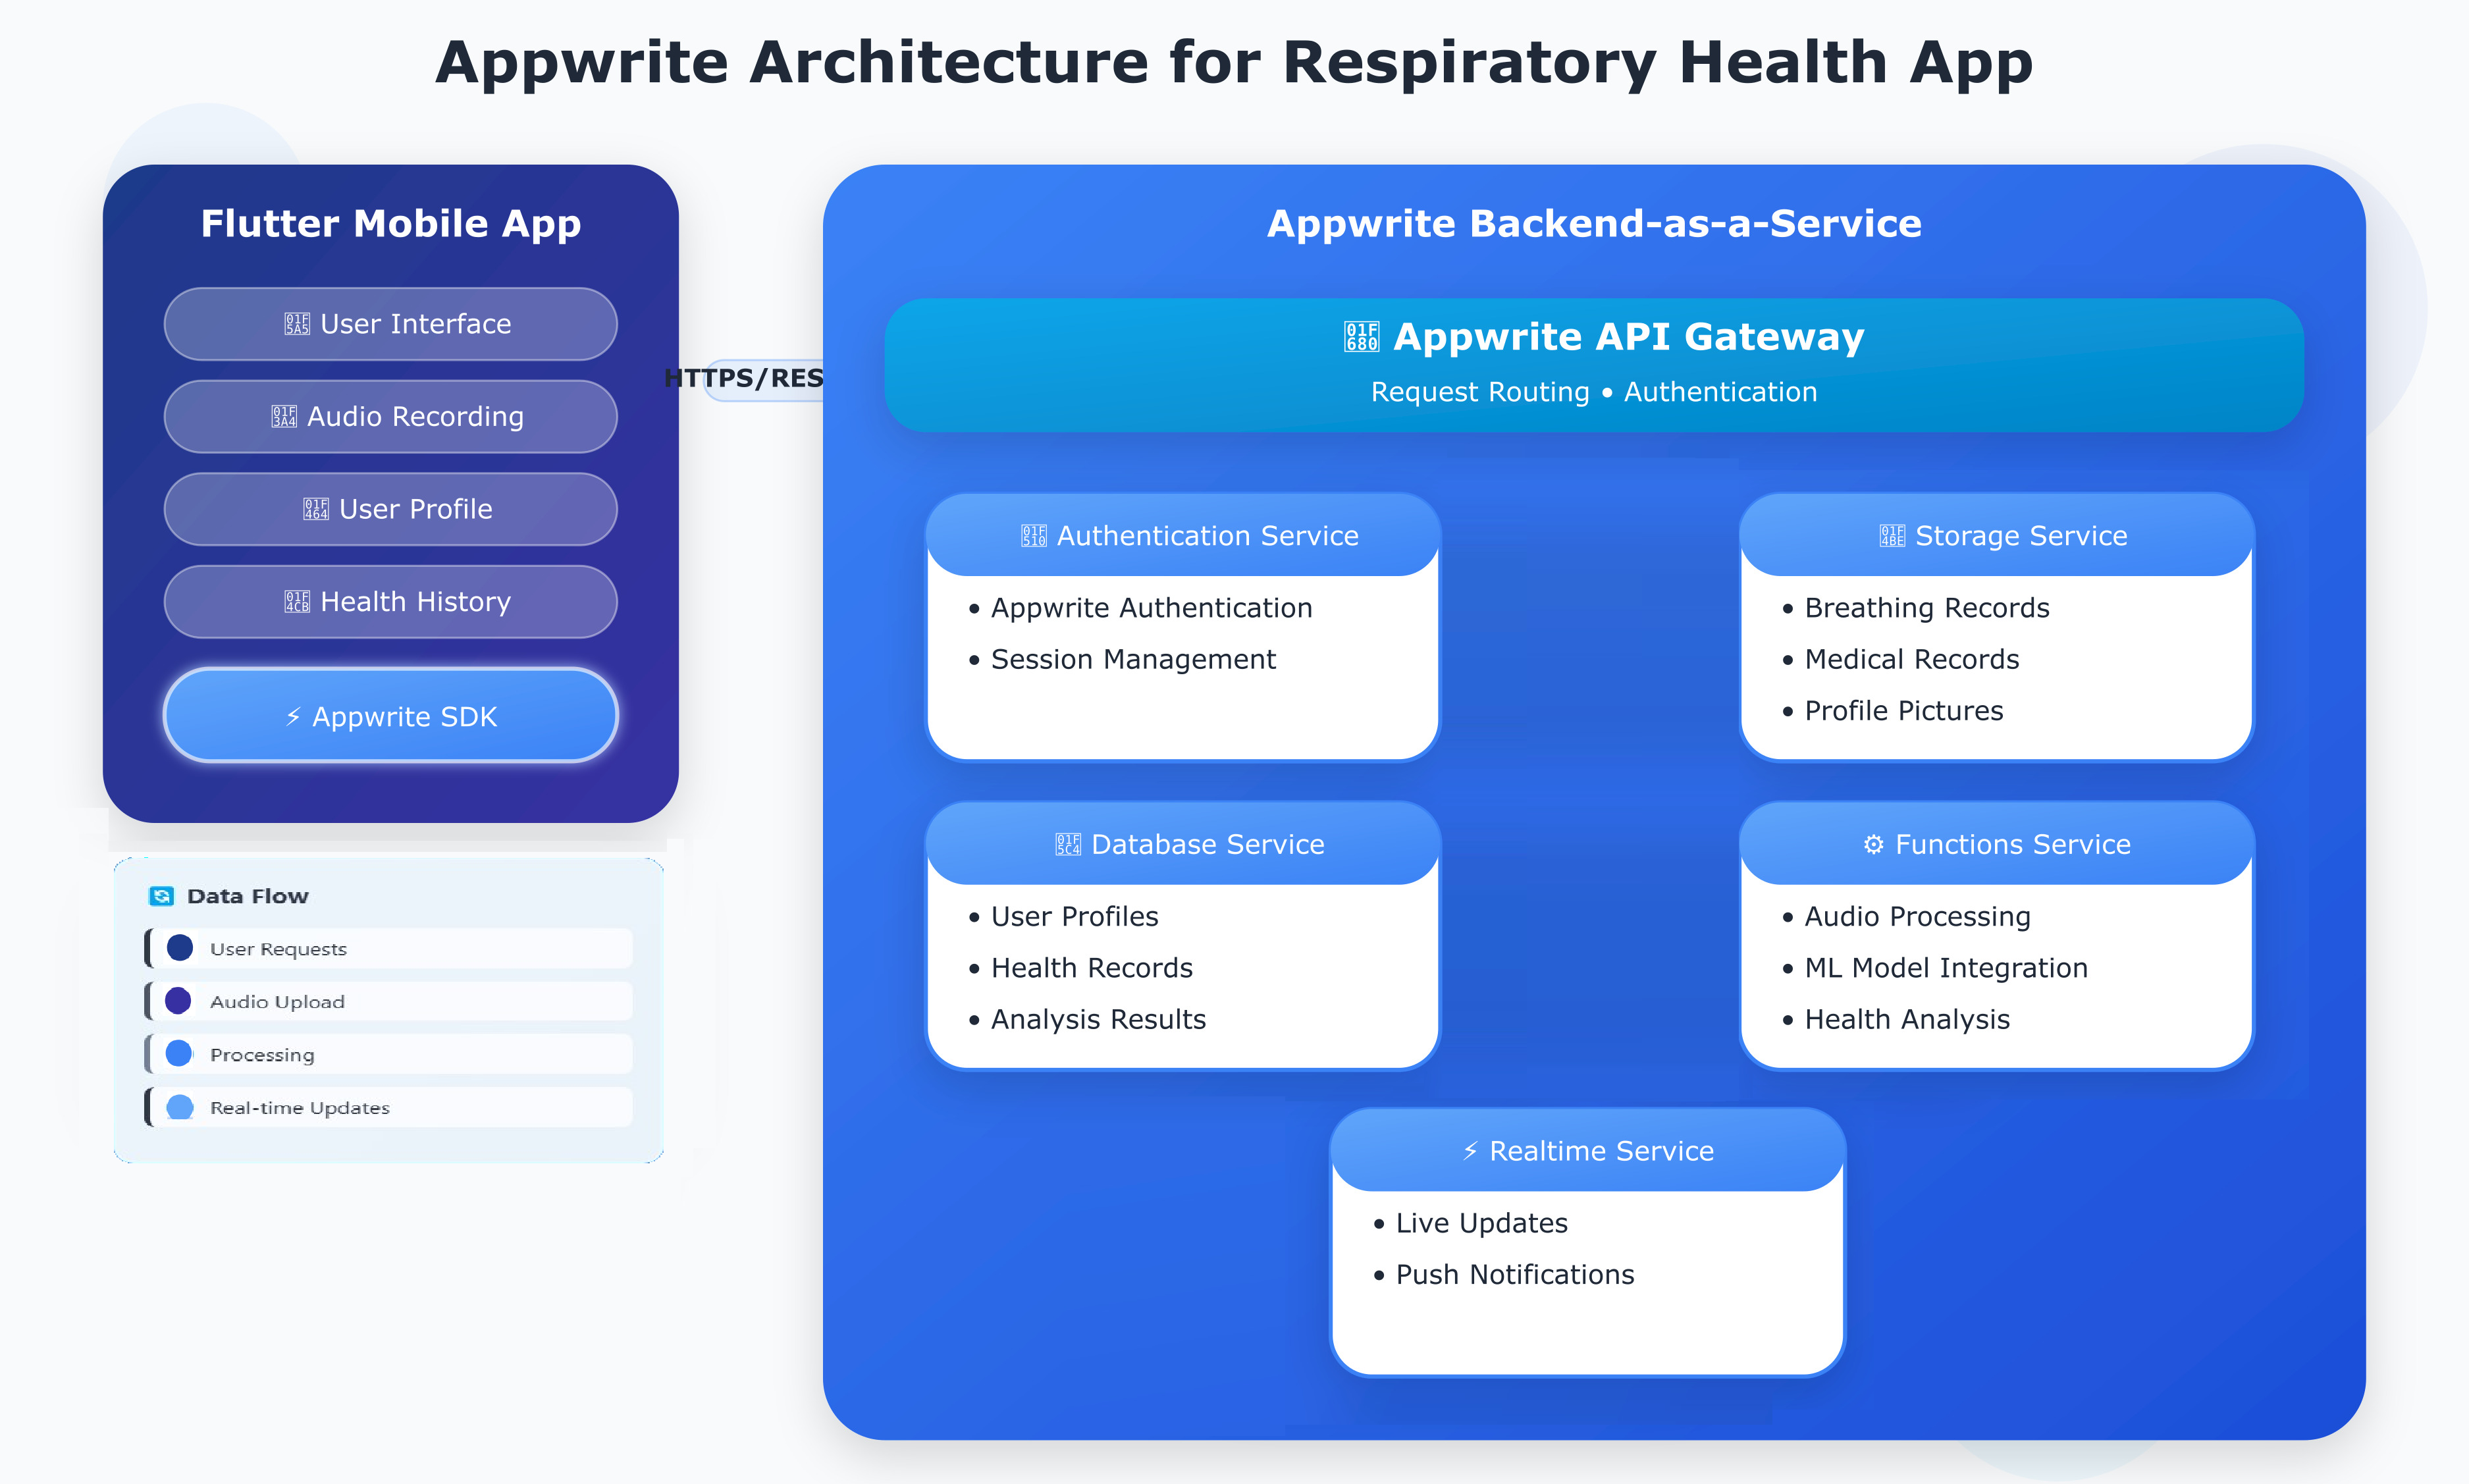
\includegraphics[width=0.95\textwidth]{images/backend/apprwite_architecture.png}
    \caption{Appwrite-Based Backend Architecture}
    \label{fig:appwrite_backend}
\end{figure}

\subsection{Authentication and Session Management}

User authentication is handled through Appwrite’s secure email-password mechanism. Upon successful login or registration, the client receives a session token, which is used to authorize all subsequent requests. This approach ensures privacy, data isolation, and secure access to personalized health information.

\subsection{Diagnosis Submission and File Handling}

When a user initiates a new diagnosis, the application uploads the audio recording and any supplementary files to Appwrite’s storage service. These assets are then linked to a new diagnosis document in the Appwrite database, which contains relevant metadata such as the timestamp, reported symptoms, and user ID.

\subsection{Triggering AI Inference}

Following submission, an Appwrite function is triggered asynchronously. This serverless function retrieves the uploaded audio file, forwards it to the AI inference engine through a secure REST API, and receives a structured JSON response. The results—comprising predicted conditions, confidence scores, and supplementary data—are saved back to the corresponding document in the database.

\subsection{Result Synchronization with the Mobile App}

To ensure responsiveness, the mobile app routinely polls the backend for updates to diagnosis records. When inference results are available, the interface updates to reflect the final diagnosis. Optionally, Appwrite’s real-time services can push changes to the client directly, allowing live updates and improved interactivity in future versions.

\subsection{Summary}

The backend architecture effectively bridges the user-facing application with the AI-driven analysis pipeline. Appwrite provides a secure, modular environment for managing identity, health data, and inference workflows. This integration enables scalable diagnostics while maintaining user privacy and system extensibility.

\section{Tools and Technologies Used}  
\label{sec:tools_tech}

The development of our AI-powered mobile diagnostic system was supported by a carefully selected suite of tools, frameworks, and platforms that together ensured efficiency, scalability, and security across the entire stack. This section introduces the core technologies employed throughout the project.

\subsection{Flutter for Cross-Platform Development}

Flutter was chosen as the core framework for building the mobile application, enabling a unified codebase for both Android and iOS platforms. Its declarative UI toolkit and reactive architecture allowed for efficient development and a smooth user experience.

The Flutter logo is shown in Figure~\ref{fig:flutter_logo}.

\begin{figure}[H]
    \centering
    
\includegraphics[width=0.25\textwidth]{images/tools/flutter.png}
    \caption{Flutter Logo}
    \label{fig:flutter_logo}
\end{figure}

\subsection{Dart Programming Language}

Dart, the language behind Flutter, was used for implementing both application logic and UI elements. Its type safety and support for asynchronous operations made it well-suited for responsive mobile development.

The Dart logo is displayed in Figure~\ref{fig:dart_logo}.

\begin{figure}[H]
    \centering
    
\includegraphics[width=0.2\textwidth]{images/tools/dart.png}
    \caption{Dart Logo}
    \label{fig:dart_logo}
\end{figure}

\subsection{Appwrite for Backend-as-a-Service}

Appwrite was selected as the backend-as-a-service solution, offering user authentication, database storage, file handling, and serverless functions. Its modular design simplified backend operations and enhanced security.

The Appwrite logo is presented in Figure~\ref{fig:appwrite_logo}.

\begin{figure}[H]
    \centering
    
\includegraphics[width=0.3\textwidth]{images/tools/appwrite.png}
    \caption{Appwrite Logo}
    \label{fig:appwrite_logo}
\end{figure}

\subsection{Python for AI Model Deployment}

Python was used to develop and deploy the AI inference engine, leveraging libraries such as PyTorch and Hugging Face Transformers for audio-based diagnosis prediction.

The Python logo can be seen in Figure~\ref{fig:python_logo}.

\begin{figure}[H]
    \centering
    
\includegraphics[width=0.25\textwidth]{images/tools/python.png}
    \caption{Python Logo}
    \label{fig:python_logo}
\end{figure}

\subsection{REST APIs for Communication}

RESTful APIs facilitated communication between the mobile frontend, Appwrite backend, and AI inference engine. This decoupled architecture allowed independent scaling and streamlined integration.

A representation of REST APIs is shown in Figure~\ref{fig:restapi_logo}.

\begin{figure}[H]
    \centering
    
\includegraphics[width=0.2\textwidth]{images/tools/restapi.png}
    \caption{REST API Representation}
    \label{fig:restapi_logo}
\end{figure}

\subsection{Docker for Containerization}

Docker was employed to containerize both Appwrite services and the AI backend. This ensured consistent deployment, streamlined development, and enhanced scalability.

The Docker logo is illustrated in Figure~\ref{fig:docker_logo}.

\begin{figure}[H]
    \centering
    
\includegraphics[width=0.3\textwidth]{images/tools/docker.png}
    \caption{Docker Logo}
    \label{fig:docker_logo}
\end{figure}

\subsection{VS Code and Postman for Development and Testing}

Visual Studio Code served as the primary development environment, providing extensive support for Dart, Flutter, and Python development.

The VS Code logo is shown in Figure~\ref{fig:vscode_logo}.

\begin{figure}[H]
    \centering
    
\includegraphics[width=0.2\textwidth]{images/tools/vscode.png}
    \caption{VS Code Logo}
    \label{fig:vscode_logo}
\end{figure}

Postman was used for testing API endpoints and simulating request flows during diagnosis.

The Postman logo is displayed in Figure~\ref{fig:postman_logo}.

\begin{figure}[H]
    \centering
    
\includegraphics[width=0.2\textwidth]{images/tools/postman.png}
    \caption{Postman Logo}
    \label{fig:postman_logo}
\end{figure}

\subsection{Android Studio for Android Emulation}

Android Studio was utilized to run the Android emulator, enabling thorough testing of the mobile application on virtual Android devices and ensuring compatibility and performance.

The Android Studio logo is shown in Figure~\ref{fig:androidstudio_logo}.

\begin{figure}[H]
    \centering
    
\includegraphics[width=0.25\textwidth]{images/tools/androidstudio.png}
    \caption{Android Studio Logo}
    \label{fig:androidstudio_logo}
\end{figure}

\subsection{Git and GitHub for Version Control}

Version control was managed using Git, with GitHub as the remote repository. This setup supported collaborative development, issue tracking, and code versioning.

The Git and GitHub logos are presented in Figure~\ref{fig:git_github_logo}.

\begin{figure}[H]
    \centering
    
\includegraphics[width=0.4\textwidth]{images/tools/git_github.png}
    \caption{Git and GitHub Logos}
    \label{fig:git_github_logo}
\end{figure}

\subsection{Summary}

The integration of these technologies ensured a robust, maintainable, and scalable solution. From frontend development to AI inference and deployment, each tool played a critical role in delivering a reliable diagnostic experience to end users.

\newpage


\section*{Conclusion}
\addcontentsline{toc}{section}{Conclusion}

\label{sec:system_summary}

This chapter provided a comprehensive overview of the system architecture and implementation details of the AI-powered mobile diagnosis application. The system is structured into three main layers: the mobile frontend, the backend infrastructure, and the AI inference engine. Each component was designed to support secure, efficient, and scalable workflows for users seeking preliminary medical feedback.

The mobile application, developed using Flutter, offers a cross-platform interface for users to describe symptoms and receive AI-generated diagnostic results. Its intuitive design and responsive UI enhance user engagement and streamline the diagnosis submission process.

The backend, powered by Appwrite, handles authentication, data storage, and serverless function execution. It acts as a secure intermediary between the mobile client and the AI inference engine, ensuring encrypted data handling, user-specific data isolation, and real-time result synchronization.

The AI pipeline, built using Python and transformer-based models, interprets audio symptom descriptions and returns structured diagnostic suggestions. It integrates seamlessly with the backend via REST APIs, enabling efficient model inference workflows.

Together, these components form a robust, modular architecture that supports accurate, secure, and real-time delivery of diagnostic information. The technology stack and integration strategy ensure future scalability, maintainability, and adaptability to more advanced diagnostic features.


\newpage

\chapter*{Conclusion and Perspectives}
\chapter*{Conclusion and Perspectives}
\addcontentsline{toc}{chapter}{Conclusion and Perspectives}
\rhead{Conclusion and Perspectives}

\section*{Conclusion}

This project presented the design and implementation of an AI-powered mobile application for breathing analysis and the detection of respiratory anomalies. The system combines mobile development with advanced AI techniques to deliver a modern, accessible diagnostic tool that supports early screening for conditions such as asthma, pneumonia, COPD, and sleep apnea.

The application allows users to record their breathing sounds, upload medical reports, and interact with an AI assistant. Through the use of Flutter for frontend development and Appwrite as a secure backend platform, the system ensures a smooth, cross-platform experience while maintaining user privacy and data integrity. On the AI side, the pipeline includes respiratory sound classification using deep learning models and personalized feedback powered by large language models (LLMs), enabling both automated diagnosis and natural language interaction.

The modular system architecture, built around RESTful APIs and containerized services, enabled seamless integration between the frontend, backend, and AI components. Tools like Docker, Git, Postman, and VS Code contributed to a robust and maintainable development workflow.

\section*{Perspectives}

While the current version of the application demonstrates the feasibility and effectiveness of AI-assisted respiratory analysis, several avenues remain for future improvement:

\begin{itemize}
  \item \textbf{Improved Audio Processing:} Incorporating advanced audio enhancement techniques, such as adaptive noise cancellation and real-time denoising, would increase the robustness of predictions in noisy environments.
  
  \item \textbf{Model Optimization and On-Device Inference:} Future iterations could explore model compression and quantization techniques to allow inference directly on the mobile device, improving response time and reducing backend dependency.

  \item \textbf{Dataset Expansion:} Increasing the diversity and size of the training dataset — including data from various age groups, devices, and environments — would improve the model’s generalization to real-world scenarios.

  \item \textbf{User Feedback Integration:} Allowing users to provide structured feedback on the accuracy of diagnoses and AI assistant responses could help continuously refine the system.

  \item \textbf{Medical Integration:} Long-term perspectives include integration with clinical workflows or partnerships with healthcare providers to support telehealth and digital triage systems.

  \item \textbf{Security and Regulatory Compliance:} Future versions should consider compliance with medical data regulations (e.g., GDPR, HIPAA) and formal security audits to ensure safe deployment in healthcare settings.
\end{itemize}

In conclusion, this project highlights the potential of combining mobile technologies with AI to support respiratory healthcare. With continued development and validation, this system can evolve into a trusted tool for early screening, patient monitoring, and AI-powered clinical assistance.



\begin{thebibliography}{10}

\bibitem{perna2019}
Perna, D., \& Tagarelli, A. (2019). 
\textit{Deep auscultation: Predicting respiratory anomalies and diseases via recurrent neural networks}. 
Proceedings of the 2019 IEEE International Conference on Bioinformatics and Biomedicine (BIBM), 2821–2827.

\bibitem{demir2021}
Demir, F., \& Sengur, A. (2021).
\textit{A deep CNN-LSTM model for classification of lung sounds}.
Biomedical Signal Processing and Control, 70, 102896.

\bibitem{ibrahim2020}
Ibrahim, A., \& Hussain, A. (2020).
\textit{Lung sound classification using recurrent neural networks and short-time Fourier transform}.
Computers in Biology and Medicine, 122, 103771.

\bibitem{aygun2022}
Aygun, M., \& Sert, E. (2022).
\textit{Respiratory sound classification using EfficientNet and spectrogram augmentation}.
IEEE Access, 10, 45329–45340.

\bibitem{icbhi2017}
Rocha, B. M., Filos, D., Mendes, L., Vogiatzis, I., Perantoni, E., Kaimakamis, E., ... \& Nascimento, J. C. (2017).
\textit{An open access database for the evaluation of respiratory sound classification algorithms}.
Physiological Measurement, 38(9), N1–N13.

\bibitem{hsu2023clap}
Hsu, W.-H., Lee, H.-Y., Yang, P.-H., Nagrani, A., Shor, J., Ferrer, L., \& Lopez Moreno, I. (2023). 
\textit{CLAP: Learning Audio-Text Joint Embeddings from Large-Scale Webly-Supervised Data}. 
arXiv preprint arXiv:2302.03102.

\bibitem{lewis2020rag}
Lewis, P., Perez, E., Piktus, A., Petroni, F., Karpukhin, V., Goyal, N., ... \& Riedel, S. (2020). 
\textit{Retrieval-Augmented Generation for Knowledge-Intensive NLP Tasks}. 
arXiv preprint arXiv:2005.11401.

\bibitem{vaswani2017attention}
Vaswani, A., Shazeer, N., Parmar, N., Uszkoreit, J., Jones, L., Gomez, A. N., Kaiser, Ł., \& Polosukhin, I. (2017).  
\textit{Attention Is All You Need}.  
Advances in Neural Information Processing Systems, 30 (NeurIPS 2017).

\bibitem{jurafsky2023slp3}
Jurafsky, D., \& Martin, J. H. (2023). 
\textit{Speech and Language Processing} (3rd ed. draft). 
Retrieved from \url{https://web.stanford.edu/~jurafsky/slp3/}

\bibitem{flutterdocs}
Google. (2023). 
\textit{Flutter Documentation}. 
Retrieved from \url{https://docs.flutter.dev/}

\bibitem{huggingface}
Hugging Face. (2023). 
\textit{Transformers Documentation}. 
Retrieved from \url{https://huggingface.co/docs/transformers/index}

\bibitem{bge2024}
Xu, Canwen, Xiao, Yixin, Ma, Yutai, Ji, Heng, \& Wang, Yining. (2024).  
\textit{BGE-M3: A Versatile Embedding Model for Retrieval, Classification, and Re-ranking}.  
arXiv preprint arXiv:2403.03692.


\end{thebibliography}


\end{document}
